\chapter{Thiết kế Giao diện và Hạ tầng Hệ thống}
\label{chap:phan4}

\section{Use Case và Yêu cầu chức năng} % Use Case Diagram + mô tả chi tiết các use case chính.
\subsection{Biểu đồ Use Case tổng thể}
Biểu đồ Use Case tổng thể của hệ thống Nền tảng Xây dựng và Mua bán Truyện tranh số được thể hiện ở Hình \ref{fig:usecase_tongthe}, được thiết kế với 4 nhóm tác nhân (actor) chính tham gia vào các module cốt lõi của nền tảng, bao gồm:
\begin{itemize}
    \item \textbf{Người dùng khách:} Tương tác chủ yếu với Module Đăng nhập/Đăng xuất để thực hiện đăng nhập và đăng ký tài khoản.
    \item \textbf{Độc giả:} Người sử dụng hệ thống để đọc truyện, mua các chương truyện trả phí và tương tác, đánh giá tác phẩm.
    \item \textbf{Tác giả:} Người sáng tạo nội dung, sử dụng hệ thống để tạo truyện, quản lý bản thảo (upload chapter, ảnh), xem dashboard thống kê và đăng bán truyện để nhận doanh thu.
    \item \textbf{Admin (Quản trị viên):} Chịu trách nhiệm quản lý người dùng và xử lý các báo cáo (reports) vi phạm trên nền tảng.
\end{itemize}

\begin{figure}[htbp]
    \centering
    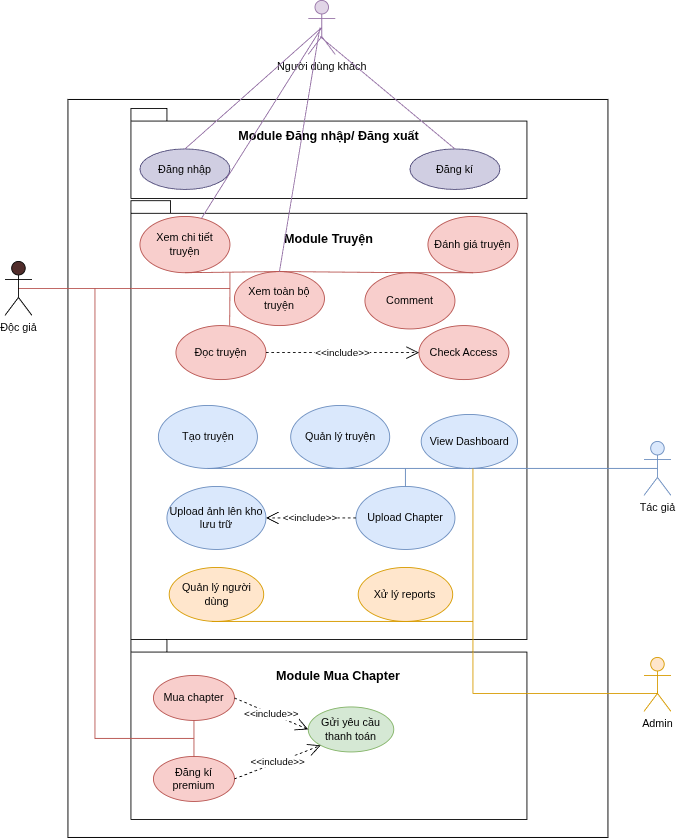
\includegraphics[width=\textwidth]{images/Diagram/use-case.png}
    \caption{Biểu đồ Use Case tổng thể của Nền tảng Xây dựng và Mua bán Truyện tranh số}
    \label{fig:usecase_tongthe}
\end{figure}

\subsection{Đặc tả chi tiết các Use Case chính}

\subsubsection{UC-01: Mua truyện}
\begin{itemize}
    \item \textbf{Tác nhân (Actor):} Độc giả.
    \item \textbf{Mô tả:} Độc giả sử dụng xu/coin trong ví để thanh toán và mở khóa các chương truyện hoặc toàn bộ bộ truyện bị khóa (trả phí).
    \item \textbf{Điều kiện tiên quyết:} Độc giả đã đăng nhập vào hệ thống và có đủ số dư xu/coin trong ví điện tử của nền tảng.
    \item \textbf{Hậu điều kiện:} Chương truyện hoặc bộ truyện được mở khóa cho tài khoản của độc giả. Số dư ví của độc giả bị trừ đi một khoản tương ứng với giá truyện.
    \item \textbf{Luồng sự kiện chính:}
    \begin{enumerate}
        \item Độc giả bấm vào một chương truyện đang bị khóa (có biểu tượng trả phí).
        \item Hệ thống hiển thị popup yêu cầu xác nhận mua chương truyện cùng mức giá.
        \item Độc giả nhấn "Xác nhận thanh toán".
        \item Hệ thống kiểm tra số dư, trừ tiền trong ví và cấp quyền truy cập nội dung.
        \item Độc giả được chuyển hướng trực tiếp vào màn hình đọc truyện.
    \end{enumerate}
    \item \textbf{Luồng thay thế:} (4a) Nếu số dư trong ví không đủ, hệ thống báo lỗi và hiển thị nút chuyển hướng sang trang "Nạp thêm xu".
    \item \textbf{Ngoại lệ:} Lỗi timeout cơ sở dữ liệu khi đang trừ tiền. Hệ thống tự động rollback giao dịch, đảm bảo tiền không bị mất và thông báo thử lại sau.
\end{itemize}

\subsubsection{UC-02: Đánh giá truyện}
\begin{itemize}
    \item \textbf{Tác nhân (Actor):} Độc giả.
    \item \textbf{Mô tả:} Người dùng viết nhận xét và chấm điểm (số sao) cho các bộ truyện mà họ đã đọc hoặc đã mua.
    \item \textbf{Điều kiện tiên quyết:} Độc giả đã đăng nhập vào hệ thống và đã đọc ít nhất một chương hoặc đã mua bộ truyện đó.
    \item \textbf{Hậu điều kiện:} Đánh giá được lưu trữ vào cơ sở dữ liệu. Điểm đánh giá trung bình của tác phẩm được cập nhật và hiển thị công khai.
    \item \textbf{Luồng sự kiện chính:}
    \begin{enumerate}
        \item Độc giả lướt xuống khu vực "Đánh giá \& phản hồi" ở cuối trang chi tiết truyện.
        \item Hệ thống hiển thị biểu mẫu (chọn từ 1 đến 5 sao, khung nhập bình luận).
        \item Độc giả chọn số sao, điền nhận xét và bấm "Gửi đánh giá".
        \item Hệ thống kiểm duyệt nội dung tự động bằng AI.
        \item Hệ thống lưu kết quả và hiển thị bình luận lên trang chi tiết của tác phẩm.
    \end{enumerate}
    \item \textbf{Luồng thay thế:} (4a) Nếu phát hiện từ ngữ vi phạm tiêu chuẩn cộng đồng, hệ thống từ chối đăng và yêu cầu người dùng chỉnh sửa lại bình luận.
    \item \textbf{Ngoại lệ:} Lỗi mất kết nối mạng khi đang gửi. Hệ thống báo lỗi và lưu tạm nội dung người dùng vừa nhập vào cache trình duyệt.
\end{itemize}

\subsubsection{UC-03: Sáng tác truyện}
\begin{itemize}
    \item \textbf{Tác nhân (Actor):} Tác giả.
    \item \textbf{Mô tả:} Tác giả tạo dự án truyện mới, cập nhật thông tin chung, tạo các chương truyện và tải lên các bản thảo/hình ảnh.
    \item \textbf{Điều kiện tiên quyết:} Người dùng đã nâng cấp/đăng ký tài khoản thành Tác giả (Creator).
    \item \textbf{Hậu điều kiện:} Thông tin dự án và các trang bản thảo được lưu trữ trên hệ thống dưới dạng "Bản nháp" (Draft).
    \item \textbf{Luồng sự kiện chính:}
    \begin{enumerate}
        \item Tác giả truy cập vào "Creator Studio Dashboard" và chọn "Tạo truyện mới".
        \item Tác giả nhập thông tin (Tên truyện, Thể loại, Tóm tắt) và tạo dự án.
        \item Tác giả chọn "Thêm chương mới" bên trong dự án.
        \item Hệ thống hiển thị trình tải lên hình ảnh (Uploader).
        \item Tác giả chọn và tải lên các trang truyện (định dạng JPG/PNG).
        \item Hệ thống sắp xếp thứ tự trang và tác giả bấm "Lưu bản nháp".
    \end{enumerate}
    \item \textbf{Luồng thay thế:} (5a) File hình ảnh tải lên vượt quá dung lượng cho phép hoặc sai định dạng. Hệ thống báo lỗi và đánh dấu đỏ vào file lỗi, yêu cầu tải lại.
    \item \textbf{Ngoại lệ:} Lỗi từ phía Server lưu trữ (Cloud Storage). Hệ thống báo lỗi tải lên thất bại và yêu cầu tác giả thử lại sau ít phút.
\end{itemize}

\subsubsection{UC-04: Đăng bán truyện}
\begin{itemize}
    \item \textbf{Tác nhân (Actor):} Tác giả.
    \item \textbf{Mô tả:} Tác giả cấu hình giá bán cho các chương truyện bản nháp và gửi yêu cầu xuất bản để đưa truyện lên Marketplace.
    \item \textbf{Điều kiện tiên quyết:} Tác giả đã có ít nhất một chương truyện lưu ở trạng thái Bản nháp và đã đồng ý với các Điều khoản chia sẻ doanh thu của nền tảng.
    \item \textbf{Hậu điều kiện:} Truyện được chuyển sang trạng thái "Công khai" (Public) hoặc "Chờ duyệt" (Pending). Độc giả có thể nhìn thấy và thực hiện mua truyện.
    \item \textbf{Luồng sự kiện chính:}
    \begin{enumerate}
        \item Trong màn hình quản lý chương truyện, tác giả chọn tính năng "Cài đặt xuất bản".
        \item Tác giả chọn chế độ "Truyện trả phí" và nhập số xu muốn bán cho chương đó.
        \item Tác giả bấm "Gửi yêu cầu xuất bản".
        \item Hệ thống kiểm tra các ràng buộc thông tin và đẩy truyện vào danh sách chờ duyệt.
        \item Sau khi quản trị viên (hoặc hệ thống tự động) duyệt thành công, truyện chính thức hiển thị trên nền tảng với mức giá đã cài đặt.
    \end{enumerate}
    \item \textbf{Luồng thay thế:} 
    \begin{itemize}
        \item (2a) Tác giả muốn cho đọc thử miễn phí: Chọn chế độ "Miễn phí", bỏ qua bước nhập giá.
        \item (5a) Truyện bị từ chối do vi phạm bản quyền: Hệ thống gửi thông báo từ chối kèm theo lý do về email của tác giả.
    \end{itemize}
    \item \textbf{Ngoại lệ:} Hệ thống cấu hình giá bị lỗi đồng bộ. Trạng thái chương truyện trả về lỗi và yêu cầu tác giả thiết lập lại.
\end{itemize}

\section{Thiết kế UI/UX}
\label{sec:uiux}

Phần UI/UX của nền tảng được thiết kế trên Figma và đã được triển khai thành prototype web. Trong bộ mockup, tên hiển thị trên giao diện là \textbf{InkVerse}; đây là tên prototype/brand UI tương ứng với hệ thống thương mại truyện tranh số \textbf{ComicFlow} đang được mô tả trong báo cáo. Việc sử dụng mockup thật giúp phần thiết kế không dừng ở mô tả ý tưởng, mà thể hiện được rõ luồng người dùng, bố cục màn hình, màu sắc, cách đặt CTA và cách hệ thống xử lý các vai trò khác nhau như độc giả, tác giả và quản trị viên.

Bộ prototype có hai nguồn tham khảo chính:

\begin{itemize}
    \item Link publish prototype: \url{https://dill-git-10102841.figma.site}
    \item Link file thiết kế Figma: \url{https://figma.com/make/hWU5734O428M0djxKt6gye/E-commerce-Comic-Platform-UI-UX}
\end{itemize}

Về định hướng trải nghiệm, ComicFlow chọn mô hình \textit{reader-first commerce}: thương mại được tích hợp vào hành trình đọc nhưng không làm gián đoạn cảm xúc thưởng thức nội dung. Người dùng mới có thể khám phá truyện, xem chi tiết và đọc thử trước khi đăng nhập; người dùng đã đăng nhập có thể lưu thư viện, nạp ví, mua chương hoặc đăng ký Premium; tác giả có dashboard riêng để đăng tải nội dung và theo dõi hiệu quả. Cách tổ chức này phù hợp với kết quả khảo sát ở Chương~\ref{chap:phan1_phan2}, trong đó người dùng quan tâm đến tốc độ tải ảnh, lưu tiến trình đọc, bình luận theo chương, tương tác với tác giả và mức giá minh bạch.

\subsection{Brand Identity và Nguyên tắc thiết kế}

Bộ nhận diện của ComicFlow/InkVerse được xây dựng theo phong cách \textit{modern fantasy digital platform}: nền tối, sắc tím chủ đạo, hiệu ứng phát sáng nhẹ và hệ thống card truyện nổi bật. Phong cách này phù hợp với sản phẩm truyện tranh số vì tạo cảm giác giải trí, trẻ trung và có tính cộng đồng, đồng thời vẫn đủ hiện đại để hỗ trợ các tác vụ thương mại như thanh toán, ví điện tử và gói Premium.

\begin{table}[H]
\centering
\caption{Định hướng brand identity thể hiện trong mockup}
\label{tab:comicflow-brand-identity-real}
\renewcommand{\arraystretch}{1.25}
\small
\begin{tabular}{|L{3.0cm}|L{4.3cm}|L{6.4cm}|}
\hline
\textbf{Thành phần} & \textbf{Thể hiện trong mockup} & \textbf{Vai trò trong trải nghiệm} \\
\hline
Màu chủ đạo
& Nền tím đậm / gần đen, kết hợp gradient tím
& Tạo không gian đọc có chiều sâu, giúp ảnh bìa truyện và các thẻ nội dung nổi bật hơn. Nền tối cũng phù hợp với thói quen đọc nội dung giải trí trong thời gian dài. \\
\hline
Màu nhấn
& Tím sáng, hồng tím, xanh cyan và vàng cho trạng thái Premium
& Dùng để nhấn CTA, tab đang chọn, thông báo, trạng thái ví và quyền lợi trả phí. Việc phân biệt màu giúp người dùng nhận ra nhanh hành động chính trên từng màn hình. \\
\hline
Typography
& Sans-serif hiện đại, chữ lớn ở hero, chữ nhỏ gọn trong card
& Bảo đảm phân cấp thông tin rõ: tiêu đề truyện, tác giả, tag thể loại, lượt xem, lượt thích và trạng thái sở hữu được đọc nhanh trong một lần quét mắt. \\
\hline
Hình ảnh
& Ảnh bìa truyện đặt trong card, hero có visual lớn
& Vì truyện tranh là sản phẩm thị giác, ảnh bìa là yếu tố kéo người dùng vào nội dung. Mockup ưu tiên card ảnh lớn thay vì mô tả chữ dài. \\
\hline
Ngôn ngữ giao diện
& Ngắn gọn, hành động rõ: Khám phá, Đọc thử, Premium, Ví, Thư viện
& Giảm thời gian học cách dùng hệ thống. Người dùng hiểu ngay mình đang khám phá, đọc, mua, quản lý thư viện hay quản lý tác phẩm. \\
\hline
\end{tabular}
\end{table}

Các nguyên tắc thiết kế chính được thể hiện trong mockup gồm:

\begin{itemize}
    \item \textbf{Content-first}: Ảnh bìa, tên truyện, tác giả, thể loại và chỉ số tương tác được đưa lên trước. Các yếu tố phụ như mô tả dài hoặc bình luận được đặt phía sau để không làm nặng màn hình khám phá.
    \item \textbf{CTA rõ ràng theo từng giai đoạn}: Ở trang chủ, CTA là khám phá truyện; ở trang chi tiết, CTA là đọc hoặc mua chương; ở màn hình Premium, CTA là chọn gói; ở dashboard tác giả, CTA là đăng truyện hoặc upload chương.
    \item \textbf{Tách vai trò người dùng}: Độc giả, tác giả và admin có giao diện riêng. Điều này giúp mỗi nhóm tập trung vào tác vụ chính của mình, tránh làm một giao diện quá nhiều chức năng.
    \item \textbf{Minh bạch thương mại}: Các màn hình ví, mua chương, thanh toán và Premium hiển thị rõ số dư, giá, quyền lợi và trạng thái giao dịch. Đây là điểm quan trọng để giảm nghi ngại khi người dùng chuyển từ đọc miễn phí sang trả phí.
    \item \textbf{Cộng đồng và tương tác}: Trang chi tiết truyện, blog, profile tác giả và bình luận theo chương tạo cảm giác nền tảng không chỉ là nơi đọc truyện, mà còn là nơi kết nối giữa độc giả và người sáng tạo.
\end{itemize}

\subsection{Mockup \& Wireframe các màn hình chính}

Bộ mockup được tổ chức theo bốn nhóm màn hình: nhóm công khai cho người dùng mới, nhóm độc giả đã đăng nhập, nhóm tác giả và nhóm quản trị. Cách chia này phản ánh đúng hành trình sản phẩm từ khám phá nội dung, đọc truyện, thanh toán, quản lý thư viện, xuất bản tác phẩm đến vận hành nền tảng.

\begin{table}[H]
\centering
\caption{Danh sách nhóm màn hình mockup và vai trò UX}
\label{tab:comicflow-main-screens-real}
\renewcommand{\arraystretch}{1.25}
\small
\begin{tabular}{|L{3.0cm}|L{4.0cm}|L{6.8cm}|}
\hline
\textbf{Nhóm màn hình} & \textbf{Màn hình chính} & \textbf{Vai trò trong hành trình người dùng} \\
\hline
Public / Guest
& Home, Explore, Comic Detail, Blog, Premium, Login
& Thu hút người dùng mới, giúp khám phá kho truyện, xem chi tiết tác phẩm, đọc nội dung cộng đồng và chuyển đổi sang đăng nhập hoặc gói trả phí. \\
\hline
Reader
& Read Chapter, Buy Comic, Payment, Library, Wallet, Profile
& Phục vụ hành vi đọc, mua chương, thanh toán, nạp ví, lưu truyện và quản lý thông tin cá nhân của độc giả. \\
\hline
Author
& Dashboard, Upload, Publish, Profile, Write Blog
& Hỗ trợ tác giả quản lý tác phẩm, đăng chương, xuất bản nội dung, viết blog và theo dõi hiệu quả hoạt động. \\
\hline
Admin
& Admin Dashboard, Settings
& Hỗ trợ quản trị nền tảng, theo dõi chỉ số vận hành, kiểm soát hệ thống, cấu hình chính sách và quản lý trạng thái nền tảng. \\
\hline
\end{tabular}
\end{table}

\subsubsection{Nhóm màn hình Public / Guest}

Nhóm màn hình công khai là điểm chạm đầu tiên của người dùng mới. Trang chủ tập trung vào hero section, danh mục truyện, truyện đang thịnh hành, truyện mới cập nhật và creator nổi bật. Trang Explore mở rộng khả năng tìm kiếm bằng bộ lọc, thể loại và danh sách truyện. Trang Comic Detail đóng vai trò như trang bán hàng cho từng tác phẩm: người dùng thấy được ảnh bìa, tác giả, thể loại, mô tả, danh sách chương, bình luận và truyện liên quan.

\begin{figure}[H]
\centering
\begin{minipage}{0.32\textwidth}
    \centering
    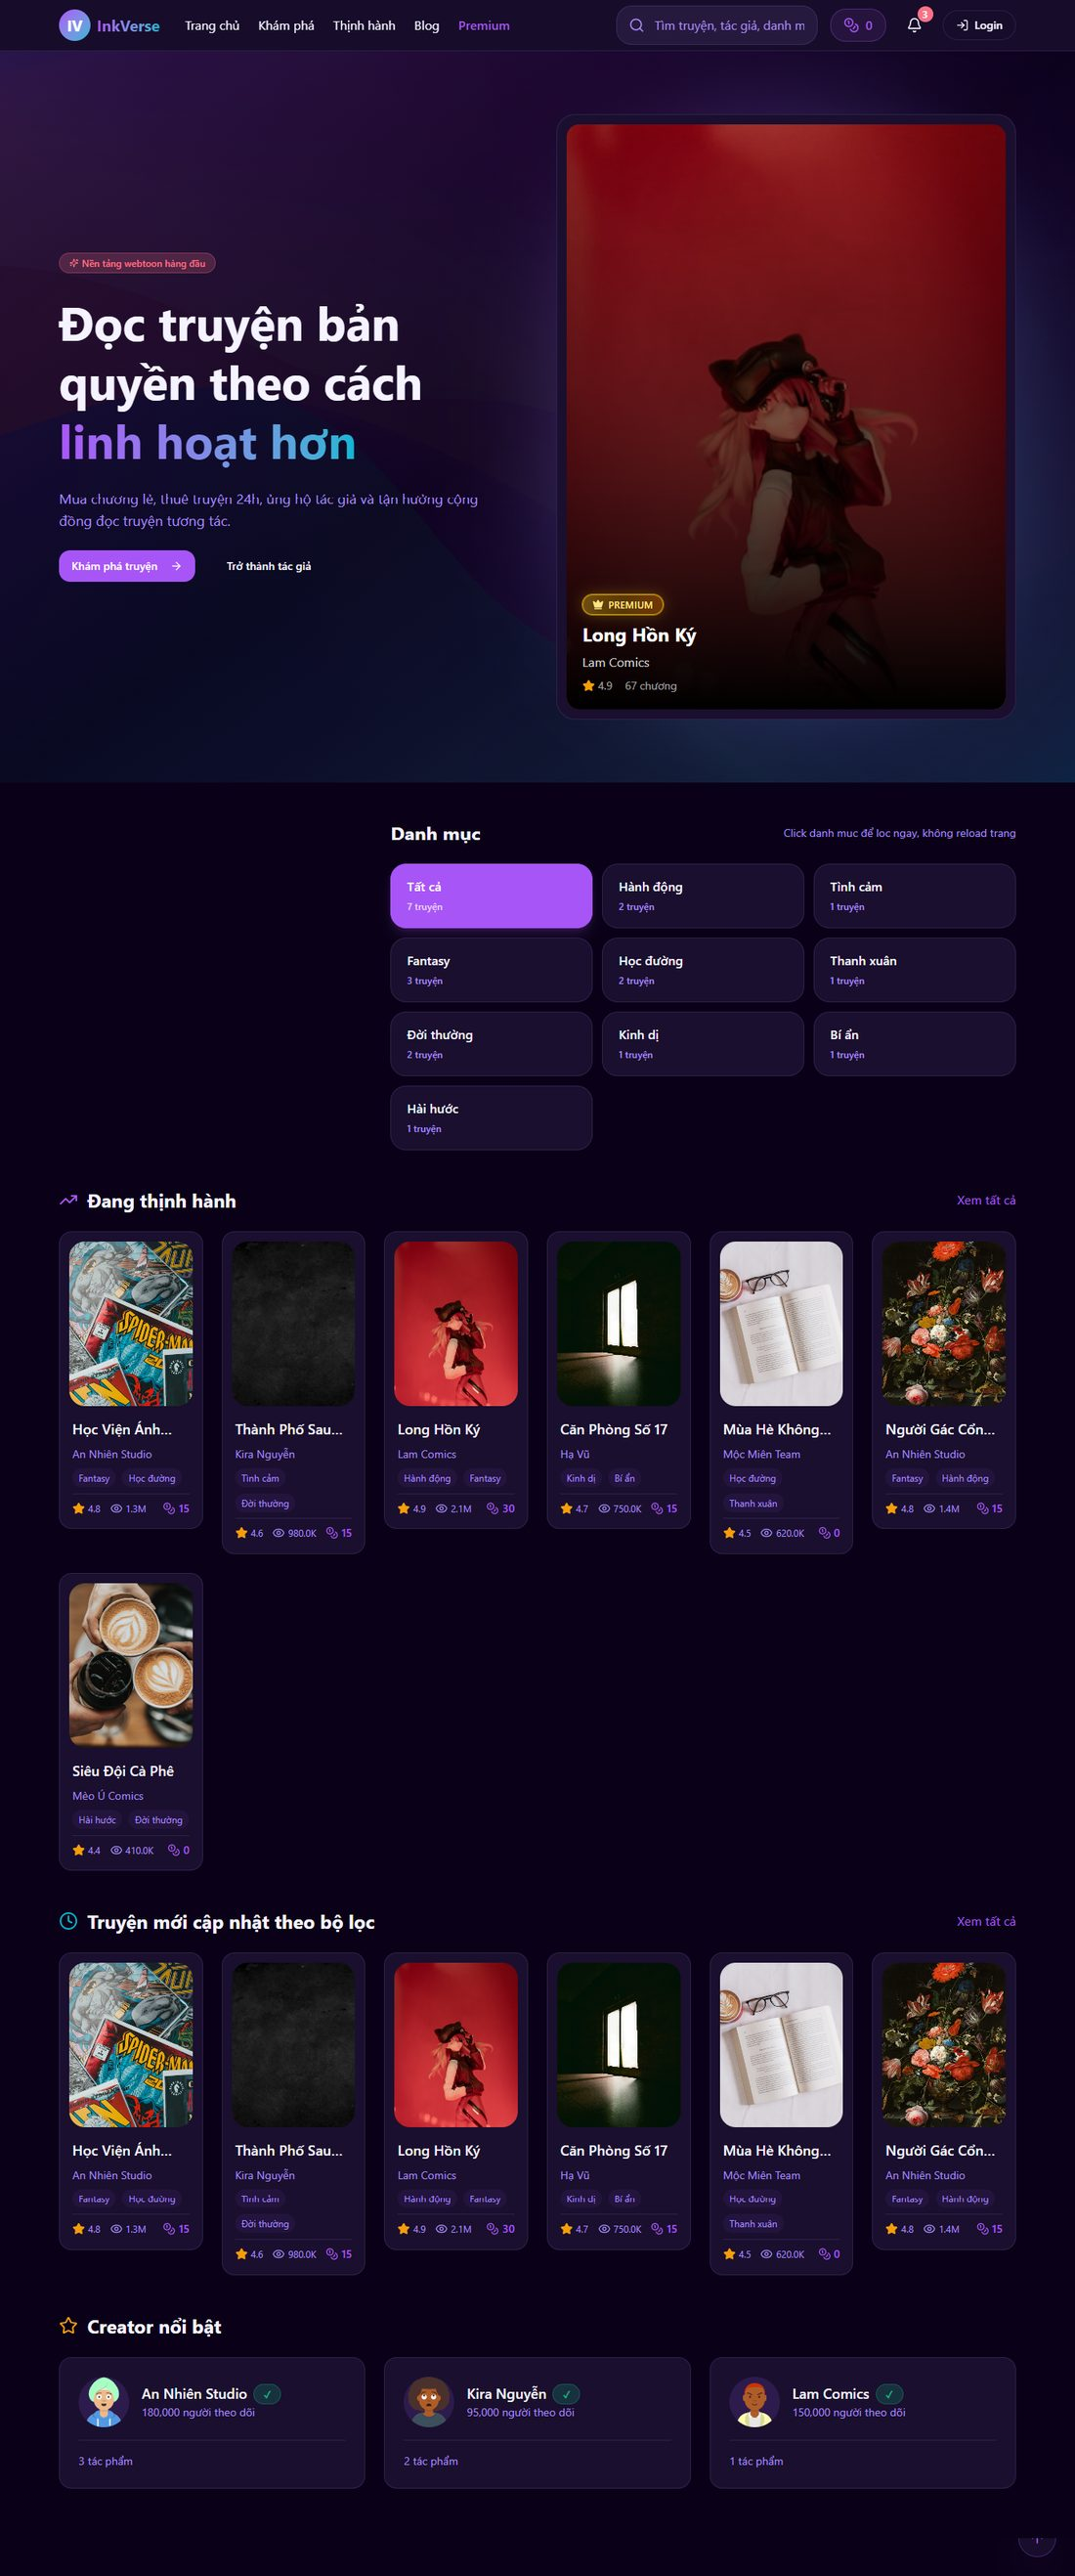
\includegraphics[width=\linewidth,height=0.31\textheight,keepaspectratio]{images/Mockups/home.jpg}
    \scriptsize Home
\end{minipage}\hfill
\begin{minipage}{0.32\textwidth}
    \centering
    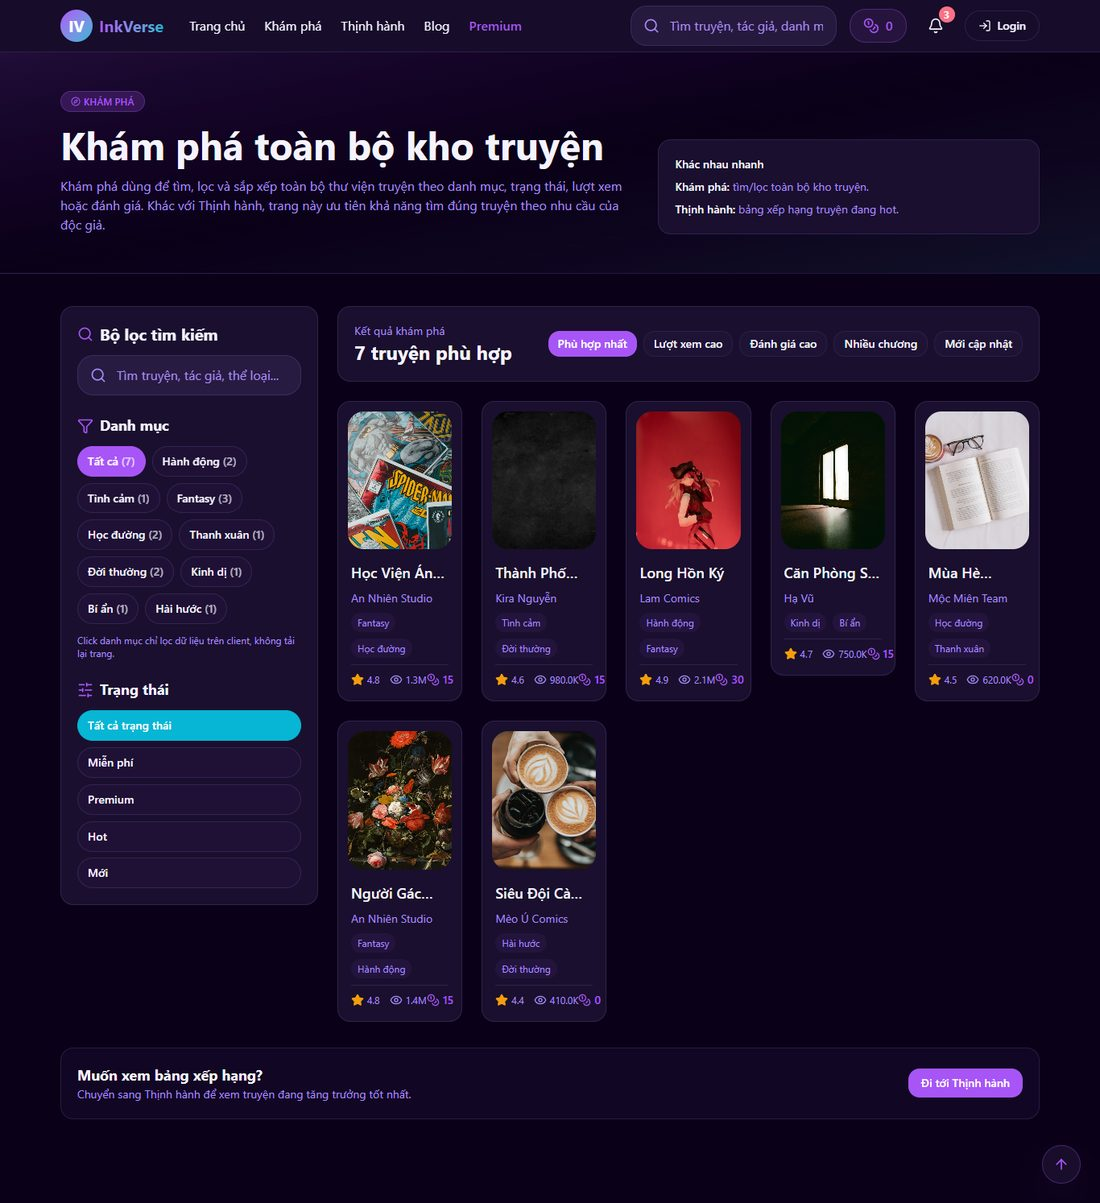
\includegraphics[width=\linewidth,height=0.31\textheight,keepaspectratio]{images/Mockups/explore.jpg}
    \scriptsize Explore
\end{minipage}\hfill
\begin{minipage}{0.32\textwidth}
    \centering
    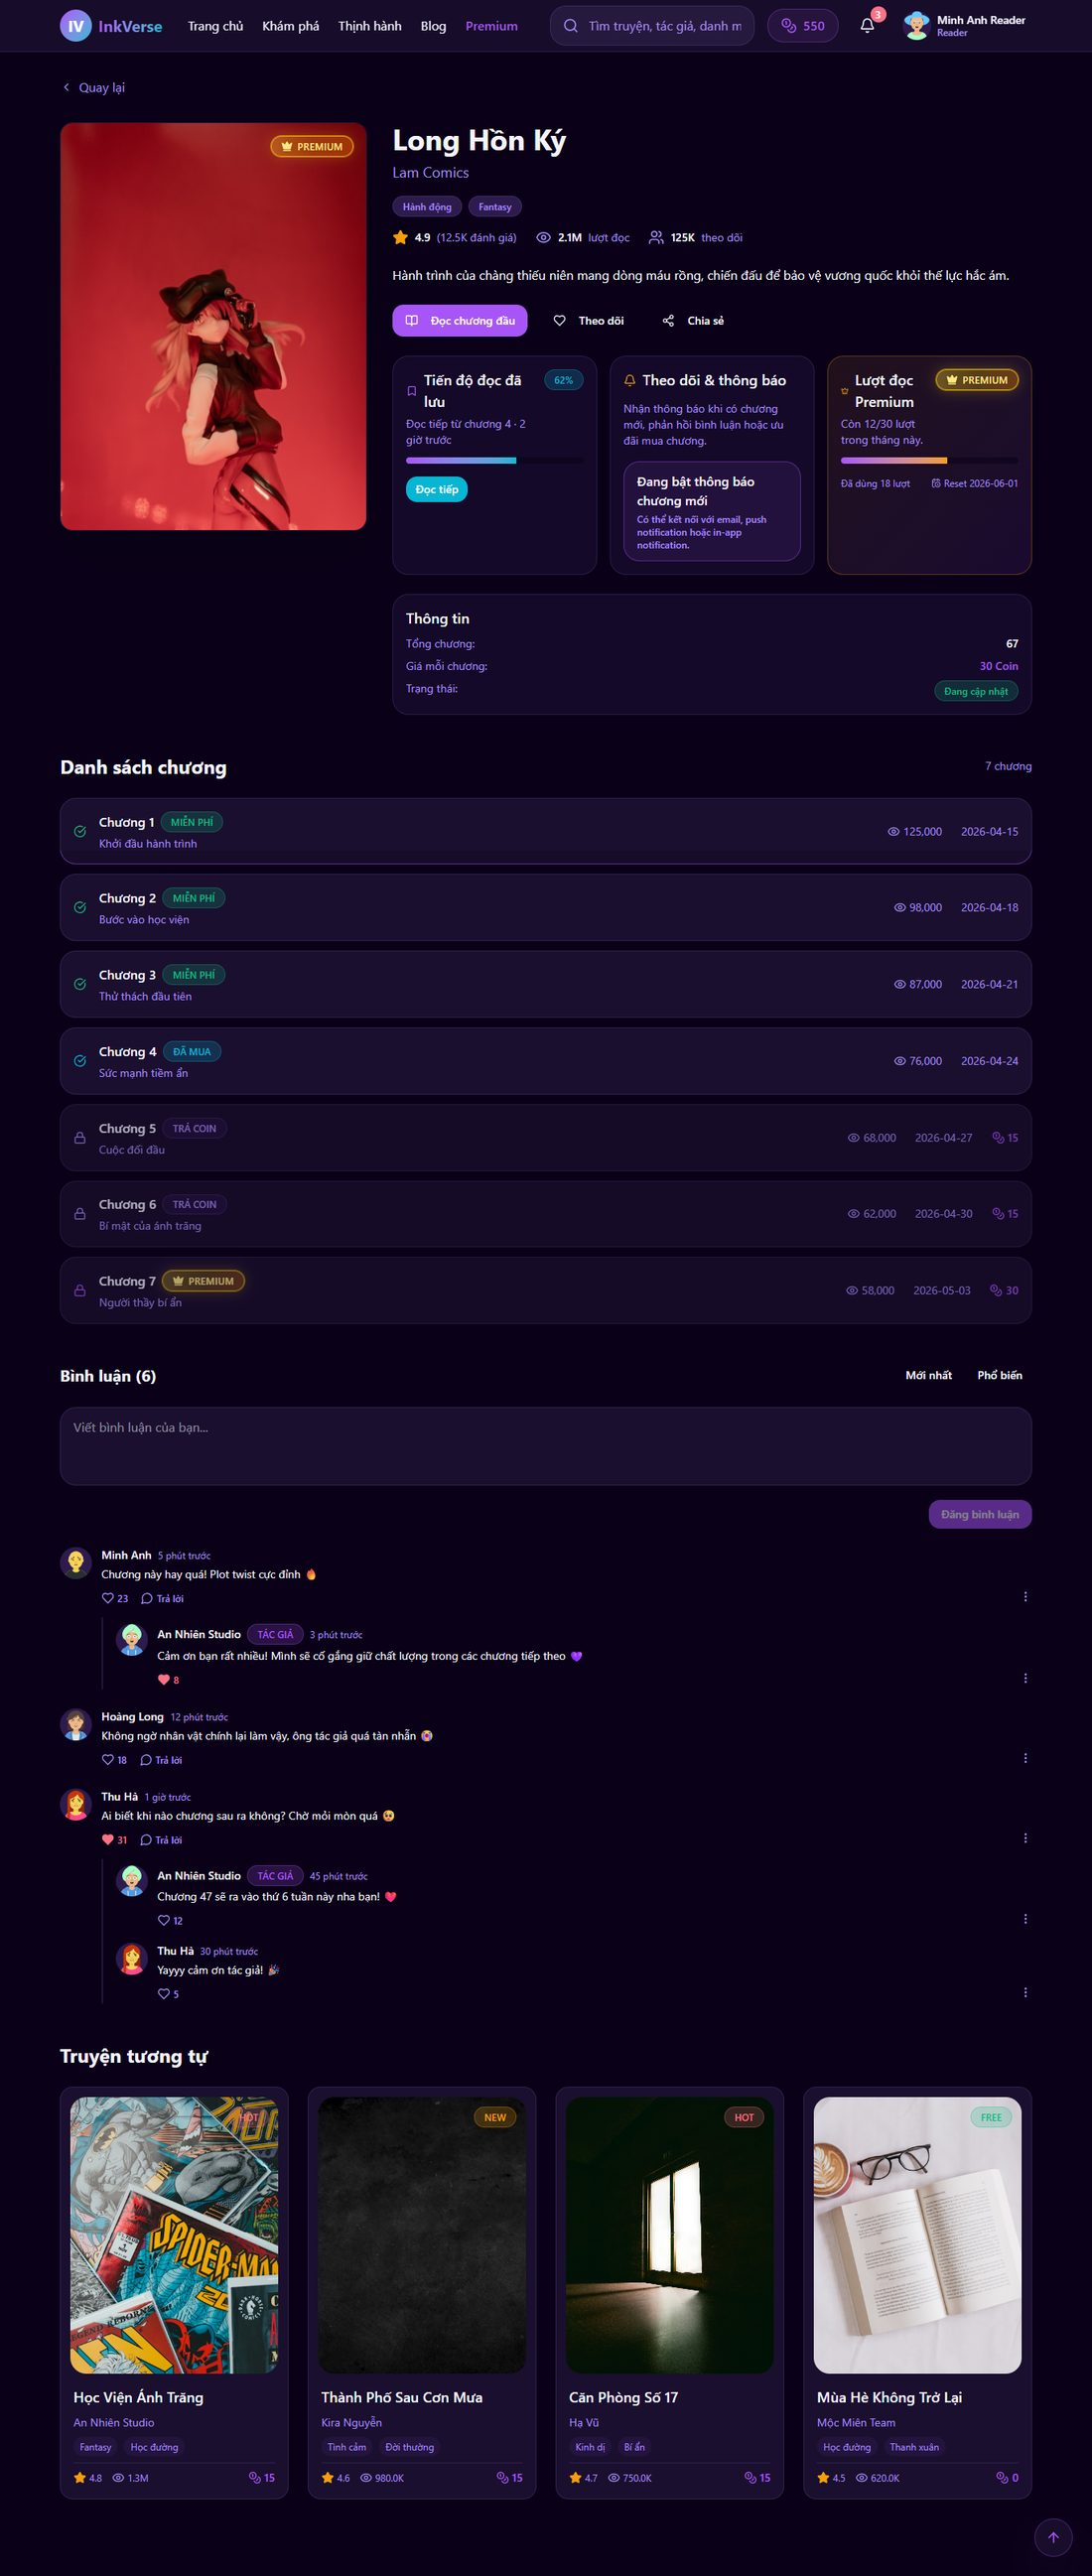
\includegraphics[width=\linewidth,height=0.31\textheight,keepaspectratio]{images/Mockups/comic_detail.jpg}
    \scriptsize Comic Detail
\end{minipage}
\caption{Mockup nhóm màn hình khám phá và chi tiết truyện}
\label{fig:mockup-public-discovery}
\end{figure}

Bố cục của nhóm màn hình này đi theo logic phễu: \textbf{Home} tạo cảm hứng, \textbf{Explore} giúp lọc và tìm truyện, còn \textbf{Comic Detail} cung cấp đủ thông tin để người dùng quyết định đọc thử, theo dõi hoặc mua chương. Điểm tốt của mockup là dùng nhiều card truyện nhất quán, có tag thể loại, chỉ số rating, lượt xem và lượt tương tác. Điều này giúp người dùng đánh giá nhanh mức hấp dẫn của truyện mà không cần vào từng trang chi tiết.

\begin{figure}[H]
\centering
\begin{minipage}{0.32\textwidth}
    \centering
    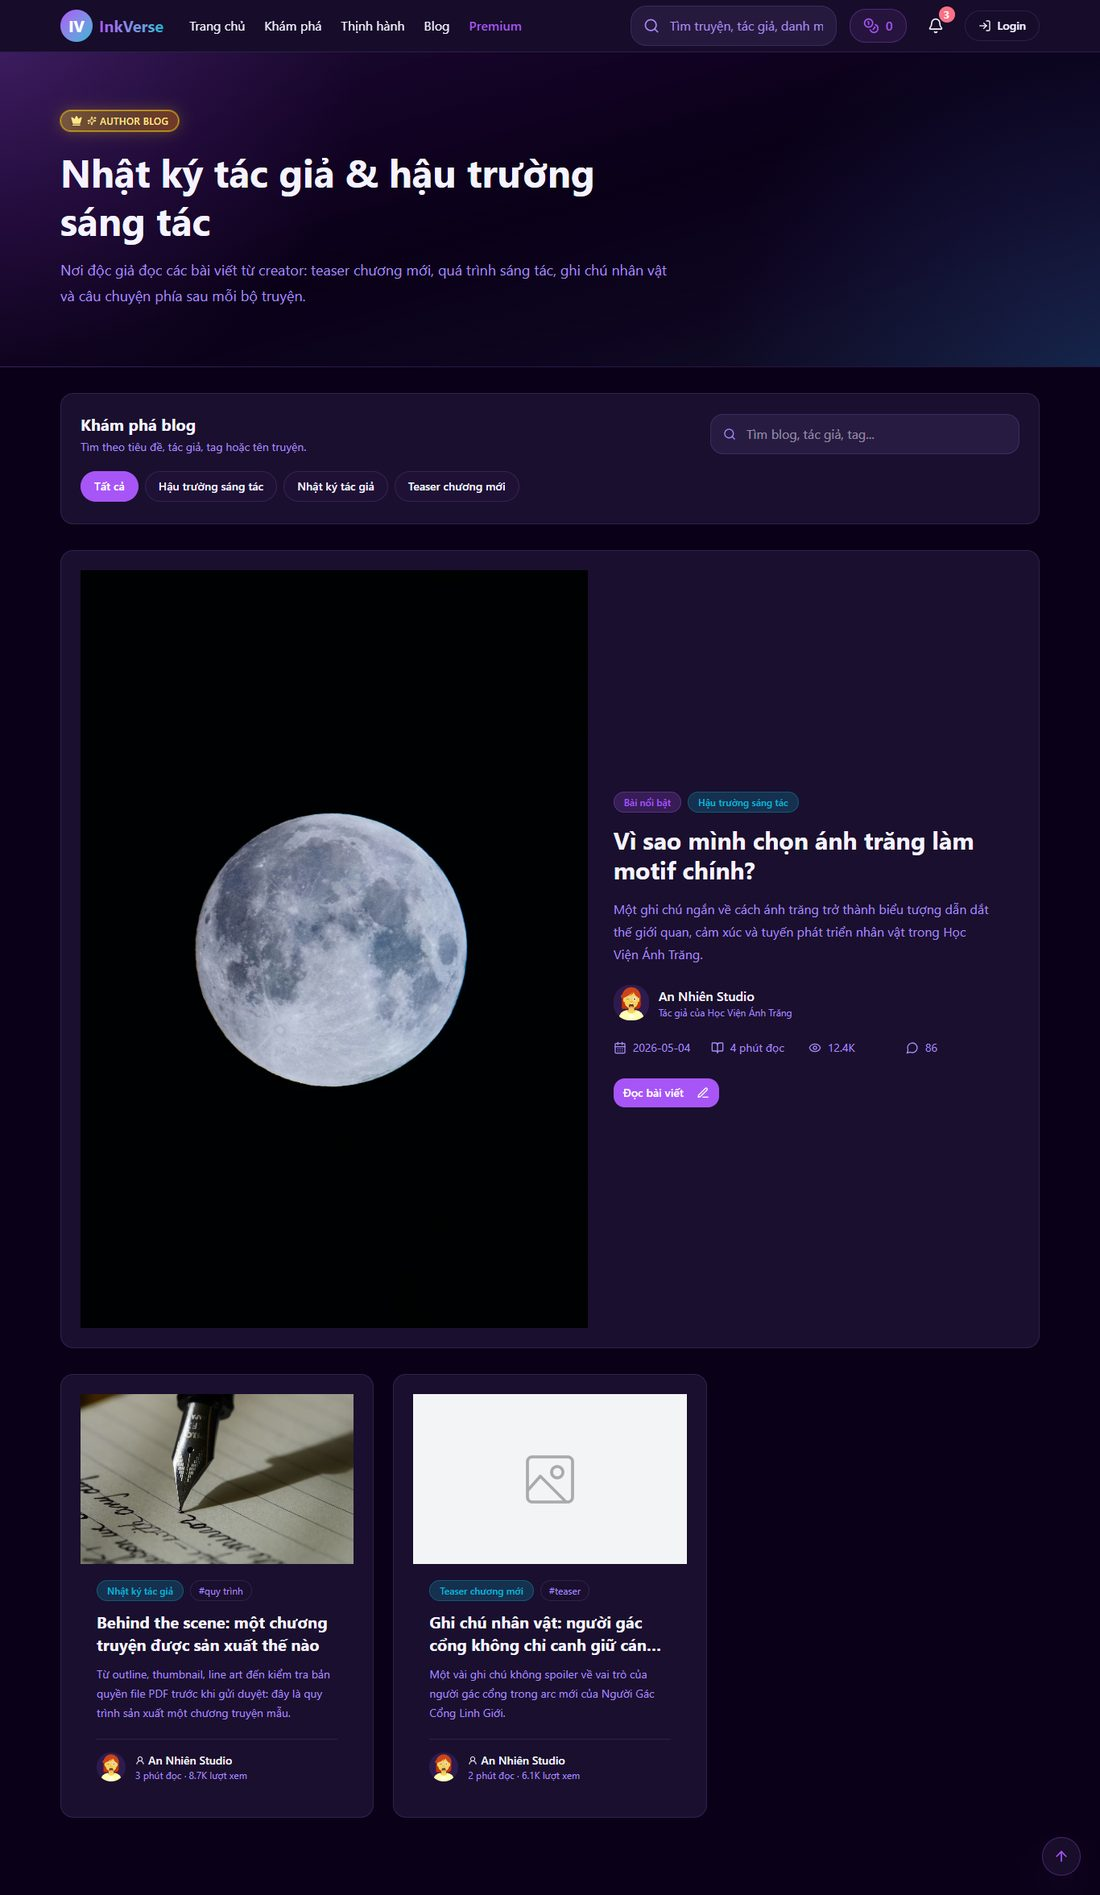
\includegraphics[width=\linewidth,height=0.29\textheight,keepaspectratio]{images/Mockups/blog.jpg}
    \scriptsize Blog cộng đồng
\end{minipage}\hfill
\begin{minipage}{0.32\textwidth}
    \centering
    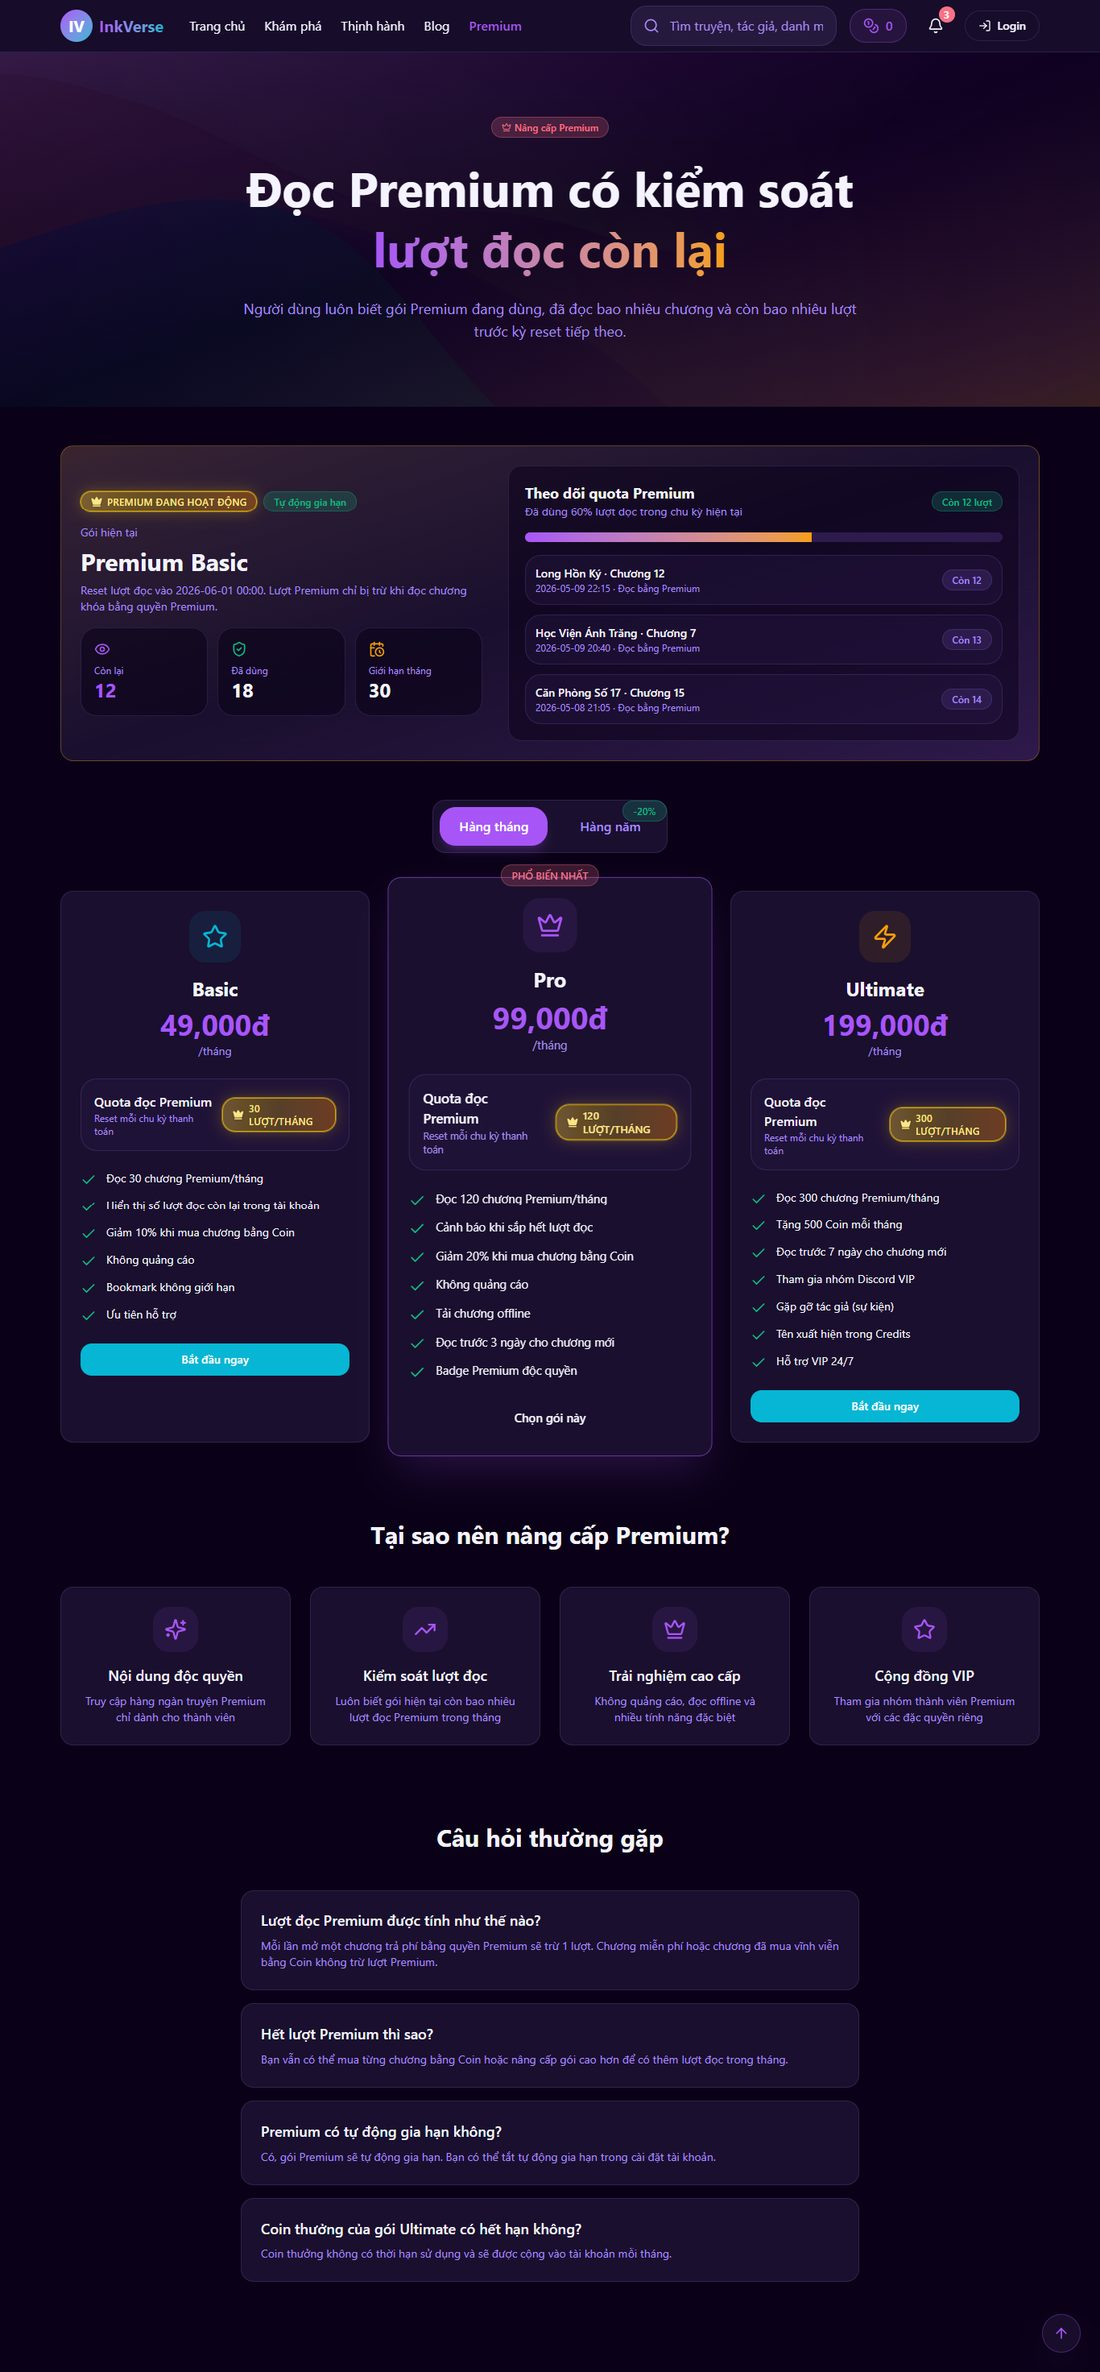
\includegraphics[width=\linewidth,height=0.29\textheight,keepaspectratio]{images/Mockups/premium.jpg}
    \scriptsize Premium
\end{minipage}\hfill
\begin{minipage}{0.32\textwidth}
    \centering
    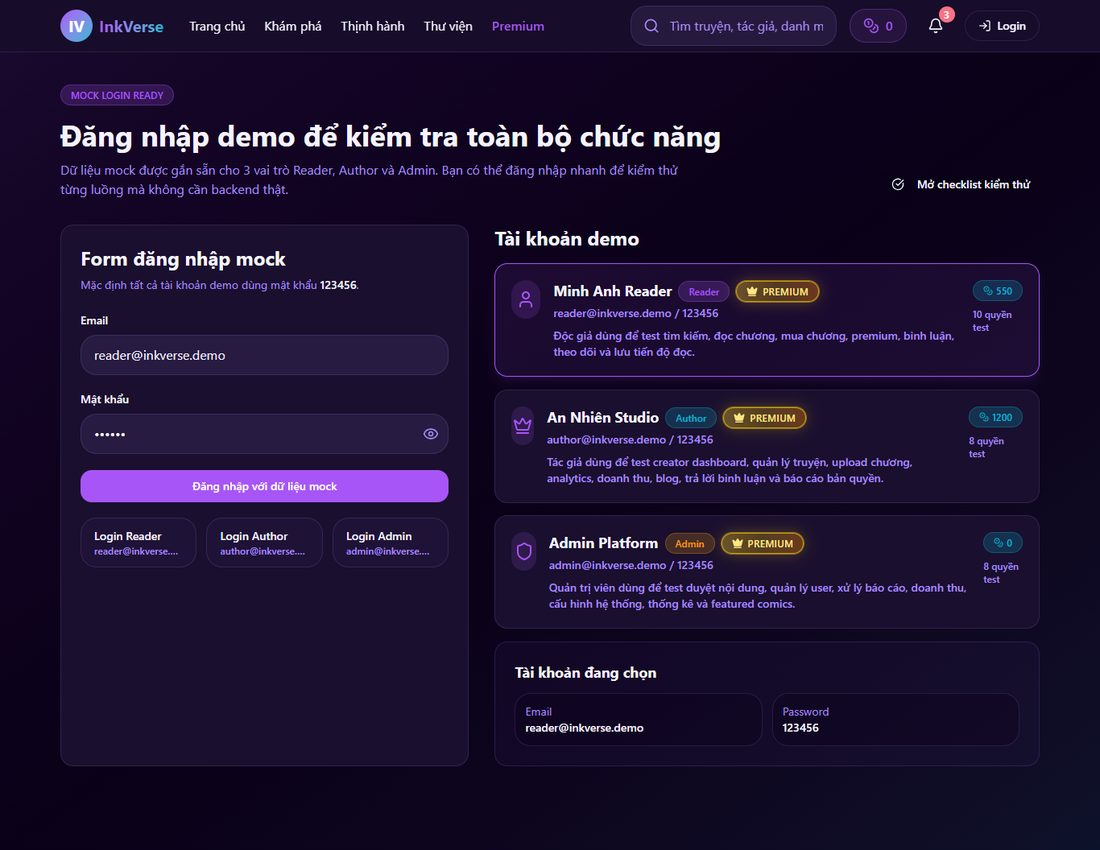
\includegraphics[width=\linewidth,height=0.29\textheight,keepaspectratio]{images/Mockups/login.jpg}
    \scriptsize Login
\end{minipage}
\caption{Mockup nhóm màn hình cộng đồng, gói trả phí và đăng nhập}
\label{fig:mockup-public-conversion}
\end{figure}

Màn hình Blog giúp nền tảng có thêm lớp nội dung cộng đồng thay vì chỉ là nơi đọc truyện. Màn hình Premium trình bày các gói quyền lợi theo card, giúp người dùng so sánh nhanh giữa các lựa chọn. Màn hình Login được thiết kế dạng form ngắn, nền tối đồng bộ với toàn hệ thống, phù hợp với nguyên tắc giảm ma sát khi chuyển đổi.

\subsubsection{Nhóm màn hình Reader}

Nhóm Reader tập trung vào các tác vụ sau khi người dùng đã có tài khoản: đọc chương, mua chương, thanh toán, quản lý thư viện, theo dõi ví và chỉnh sửa hồ sơ. Đây là nhóm màn hình ảnh hưởng trực tiếp đến retention và doanh thu, vì trải nghiệm đọc không tốt hoặc thanh toán không rõ ràng sẽ làm người dùng rời bỏ rất nhanh.

\begin{figure}[H]
\centering
\begin{minipage}{0.32\textwidth}
    \centering
    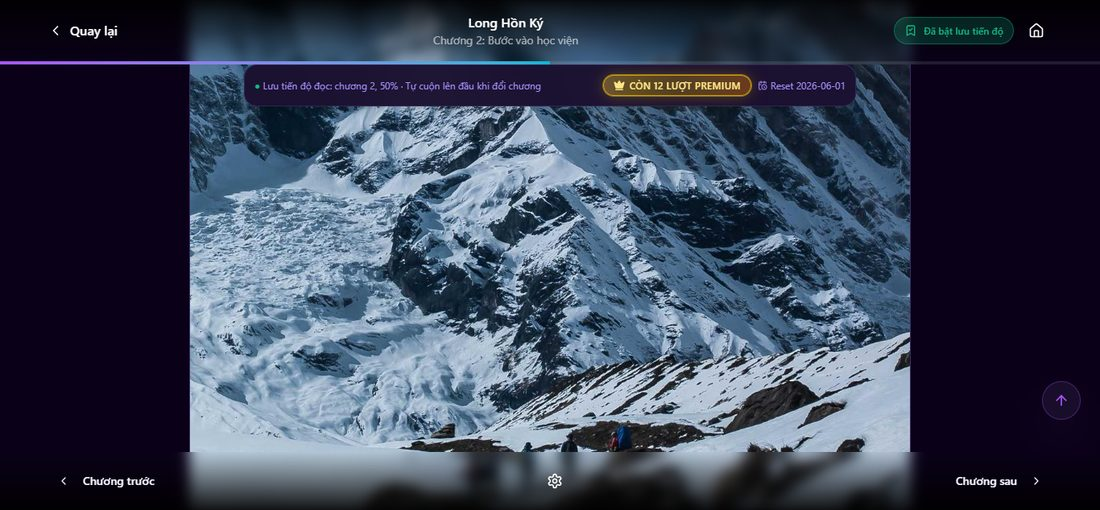
\includegraphics[width=\linewidth,height=0.25\textheight,keepaspectratio]{images/Mockups/reader_read_chapter.jpg}
    \scriptsize Read Chapter
\end{minipage}\hfill
\begin{minipage}{0.32\textwidth}
    \centering
    
\includegraphics[width=\linewidth,height=0.25\textheight,keepaspectratio]{images/Mockups/reader_buy_comic.jpg}
    \scriptsize Buy Comic
\end{minipage}\hfill
\begin{minipage}{0.32\textwidth}
    \centering
    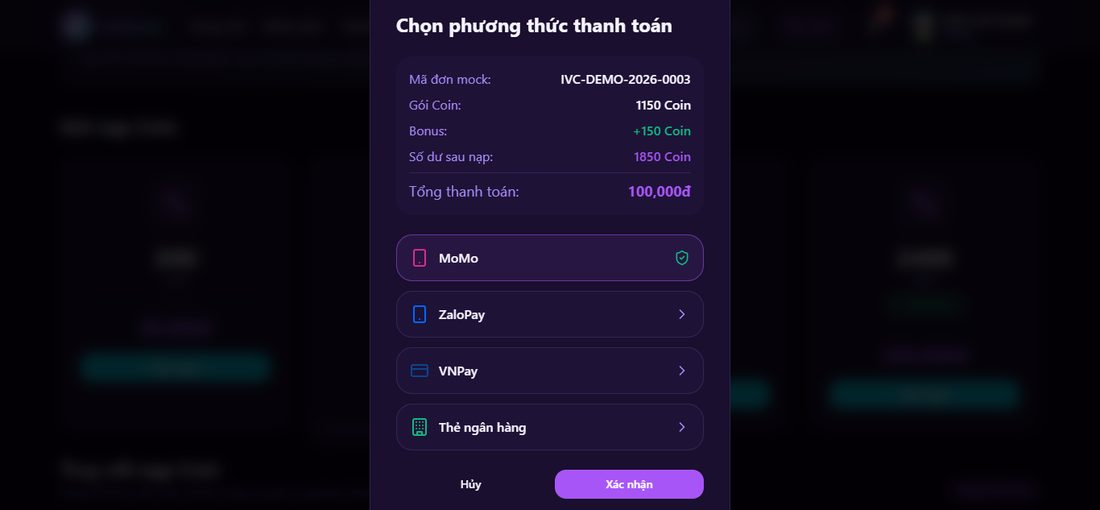
\includegraphics[width=\linewidth,height=0.25\textheight,keepaspectratio]{images/Mockups/reader_payment.jpg}
    \scriptsize Payment
\end{minipage}
\caption{Mockup luồng đọc truyện, mua chương và thanh toán}
\label{fig:mockup-reader-payment}
\end{figure}

Màn hình đọc chương được tối giản để nội dung truyện là trung tâm. Các thao tác phụ như điều hướng chương, mở menu, mua chương hoặc quay lại được đặt xung quanh vùng đọc. Modal Buy Comic hiển thị thông tin giao dịch ngay tại ngữ cảnh đọc, giúp người dùng không bị kéo ra khỏi trải nghiệm chính. Màn hình Payment tiếp tục luồng mua với thông tin số tiền và trạng thái xác nhận rõ ràng.

\begin{figure}[H]
\centering
\begin{minipage}{0.32\textwidth}
    \centering
    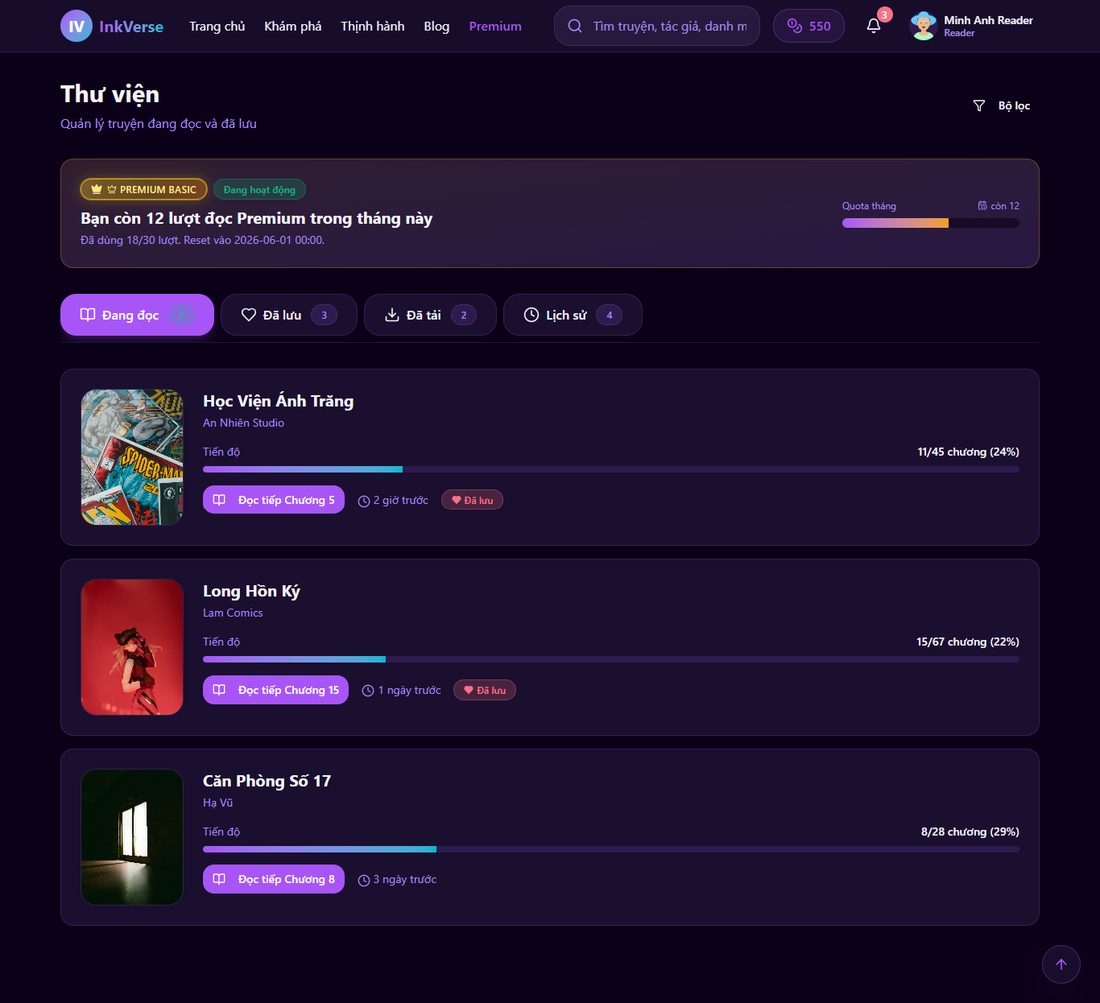
\includegraphics[width=\linewidth,height=0.31\textheight,keepaspectratio]{images/Mockups/reader_library.jpg}
    \scriptsize Library
\end{minipage}\hfill
\begin{minipage}{0.32\textwidth}
    \centering
    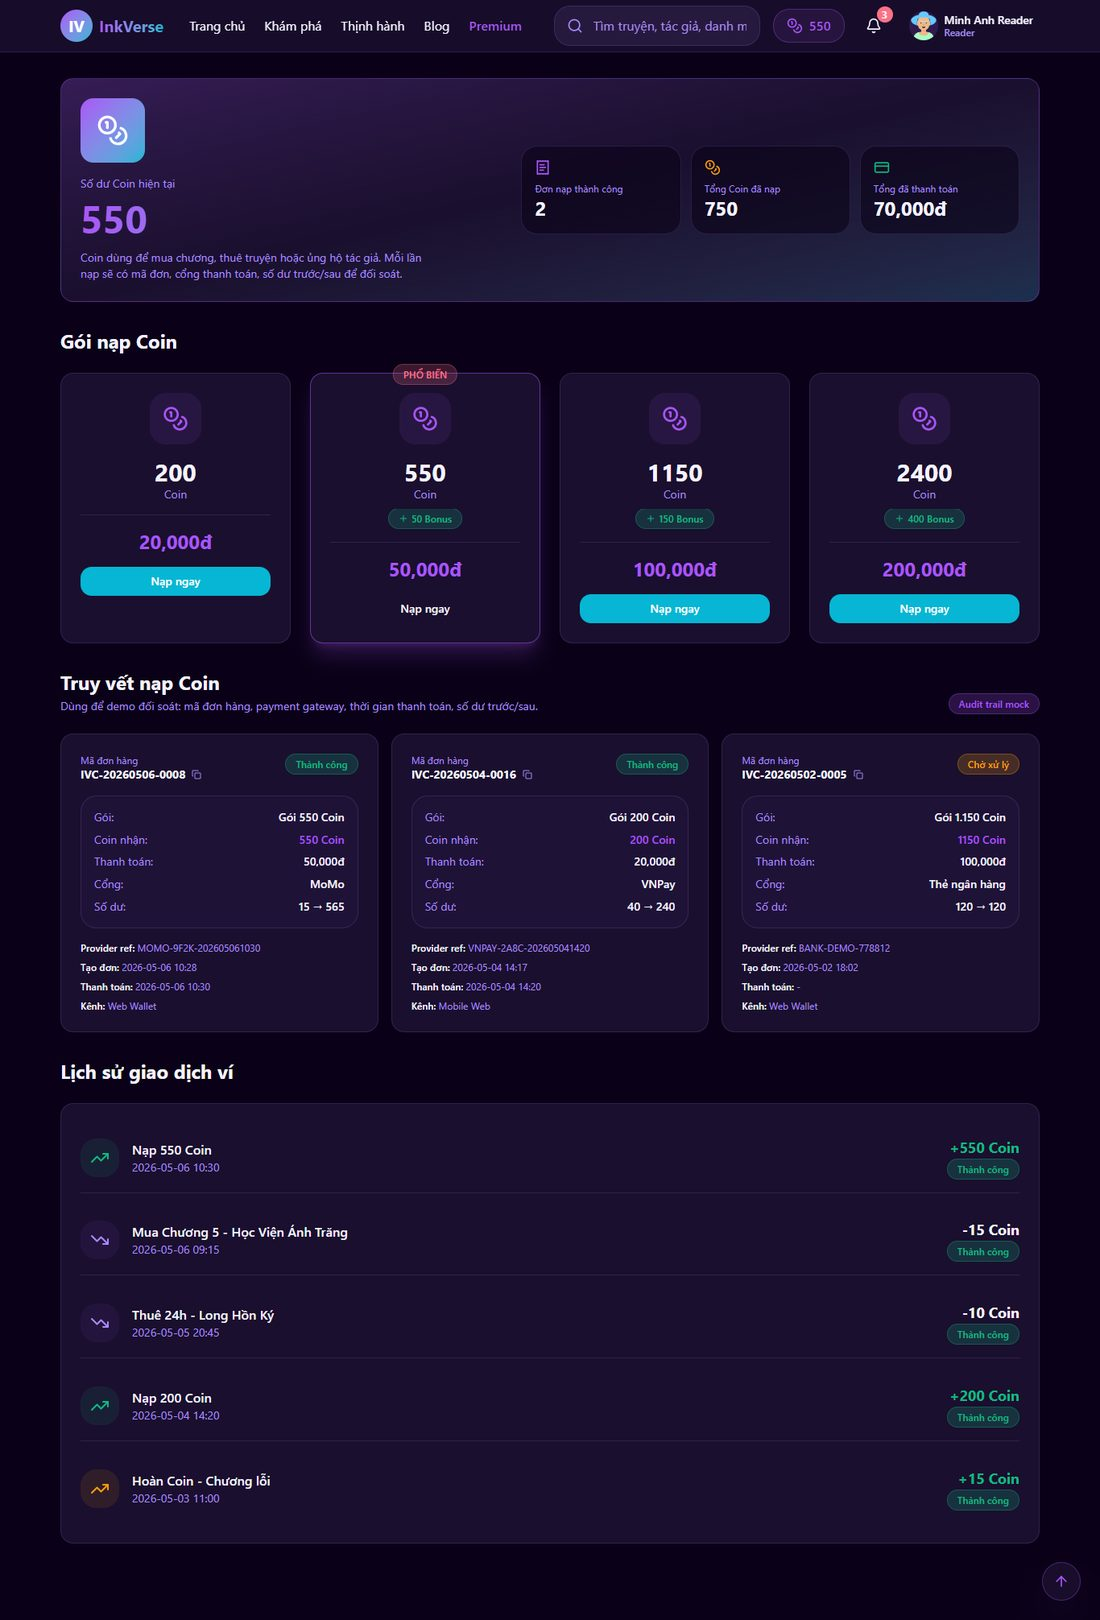
\includegraphics[width=\linewidth,height=0.31\textheight,keepaspectratio]{images/Mockups/reader_wallet.jpg}
    \scriptsize Wallet
\end{minipage}\hfill
\begin{minipage}{0.32\textwidth}
    \centering
    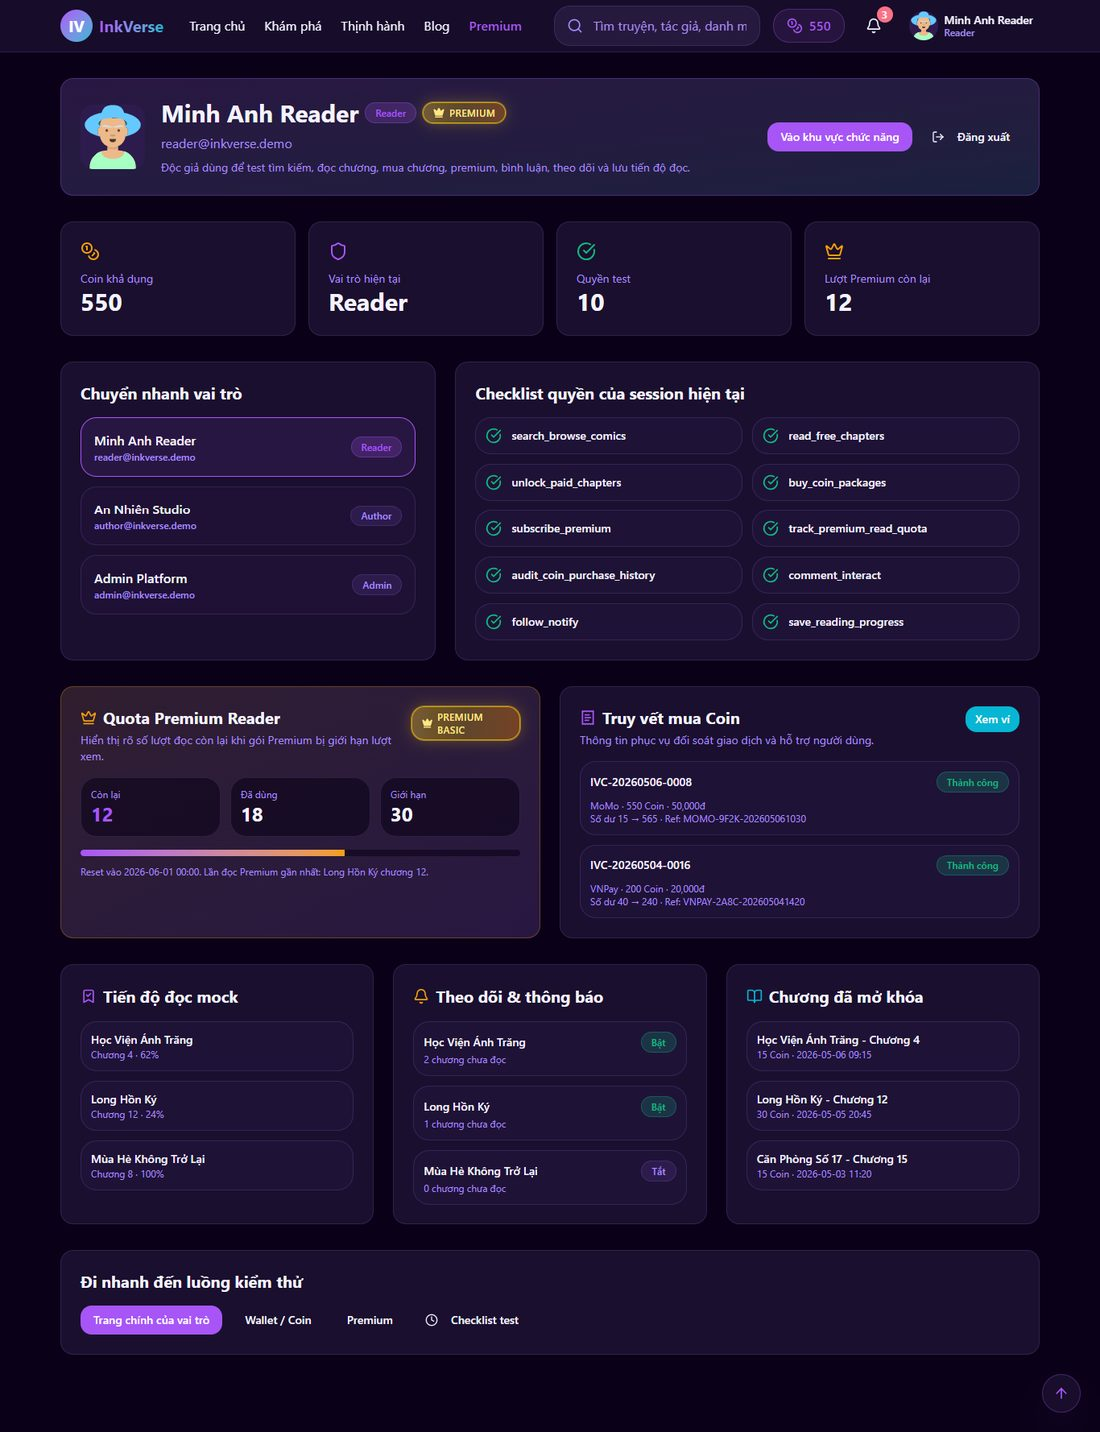
\includegraphics[width=\linewidth,height=0.31\textheight,keepaspectratio]{images/Mockups/reader_profile.jpg}
    \scriptsize Reader Profile
\end{minipage}
\caption{Mockup nhóm màn hình quản lý tài khoản độc giả}
\label{fig:mockup-reader-account}
\end{figure}

Thư viện cá nhân giúp người đọc quay lại các truyện đang theo dõi hoặc đã mua. Ví điện tử hiển thị số dư, lịch sử giao dịch và các gói nạp, đóng vai trò cầu nối giữa hành vi đọc và hành vi thanh toán. Profile độc giả tổng hợp thông tin tài khoản, hoạt động đọc và các tuỳ chọn cá nhân, giúp tăng cảm giác sở hữu tài khoản trên nền tảng.

\subsubsection{Nhóm màn hình Author}

Nhóm Author được thiết kế cho người sáng tạo nội dung. Đây là điểm khác biệt quan trọng so với các trang đọc truyện không bản quyền, vì nền tảng không chỉ cần người đọc mà còn phải tạo động lực cho tác giả đăng tải và duy trì nội dung. Dashboard tác giả cần cho thấy hiệu quả xuất bản thông qua số liệu, trong khi các màn hình Upload và Publish giúp quá trình đăng truyện trở nên rõ ràng, có trạng thái và ít lỗi.

\begin{figure}[H]
\centering
\begin{minipage}{0.32\textwidth}
    \centering
    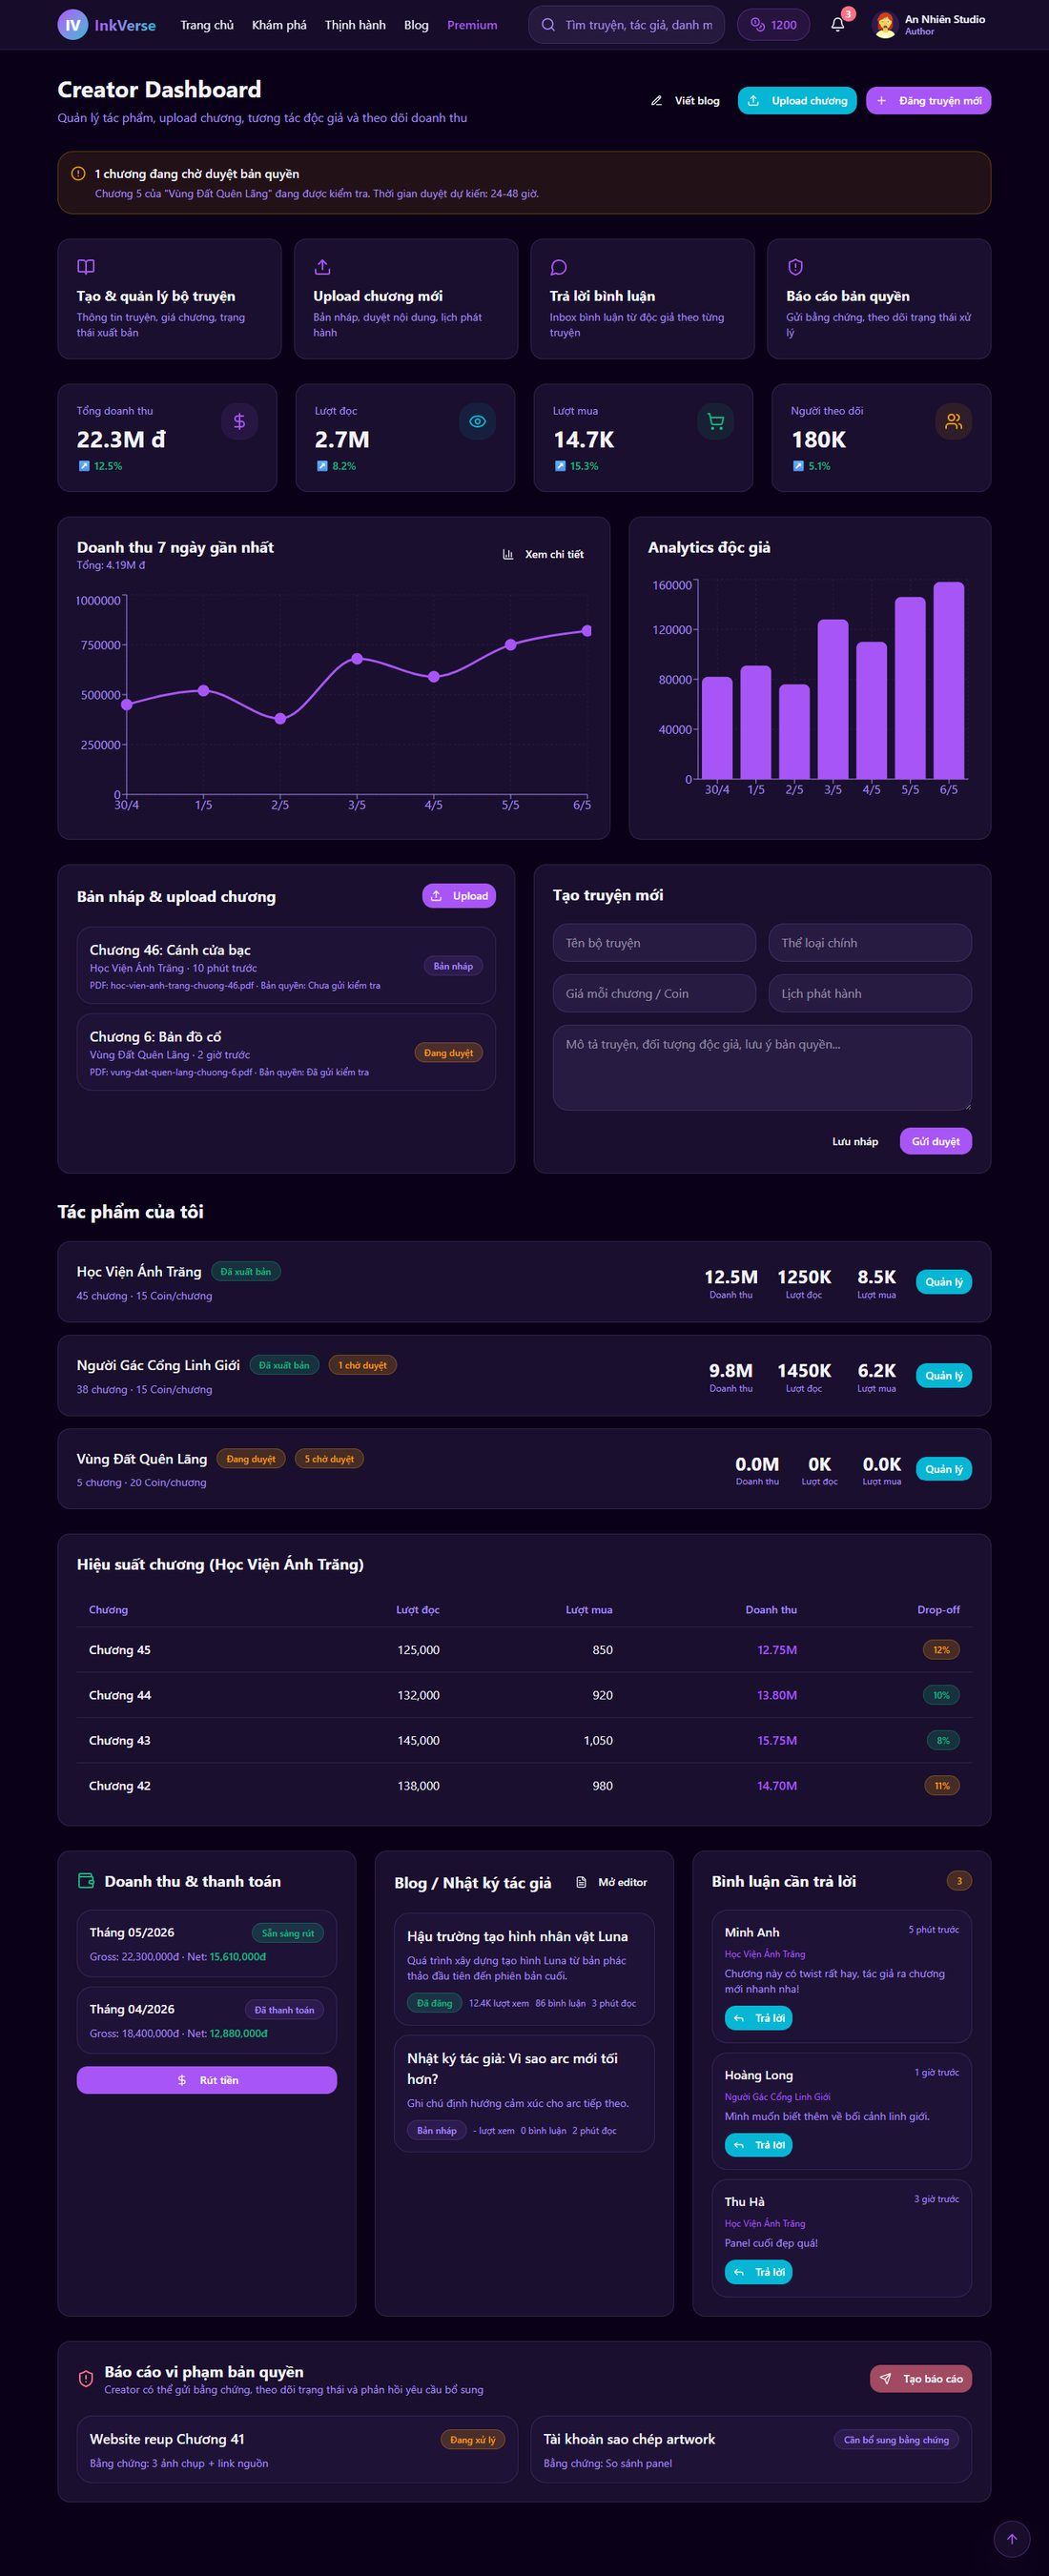
\includegraphics[width=\linewidth,height=0.31\textheight,keepaspectratio]{images/Mockups/author_dashboard.jpg}
    \scriptsize Author Dashboard
\end{minipage}\hfill
\begin{minipage}{0.32\textwidth}
    \centering
    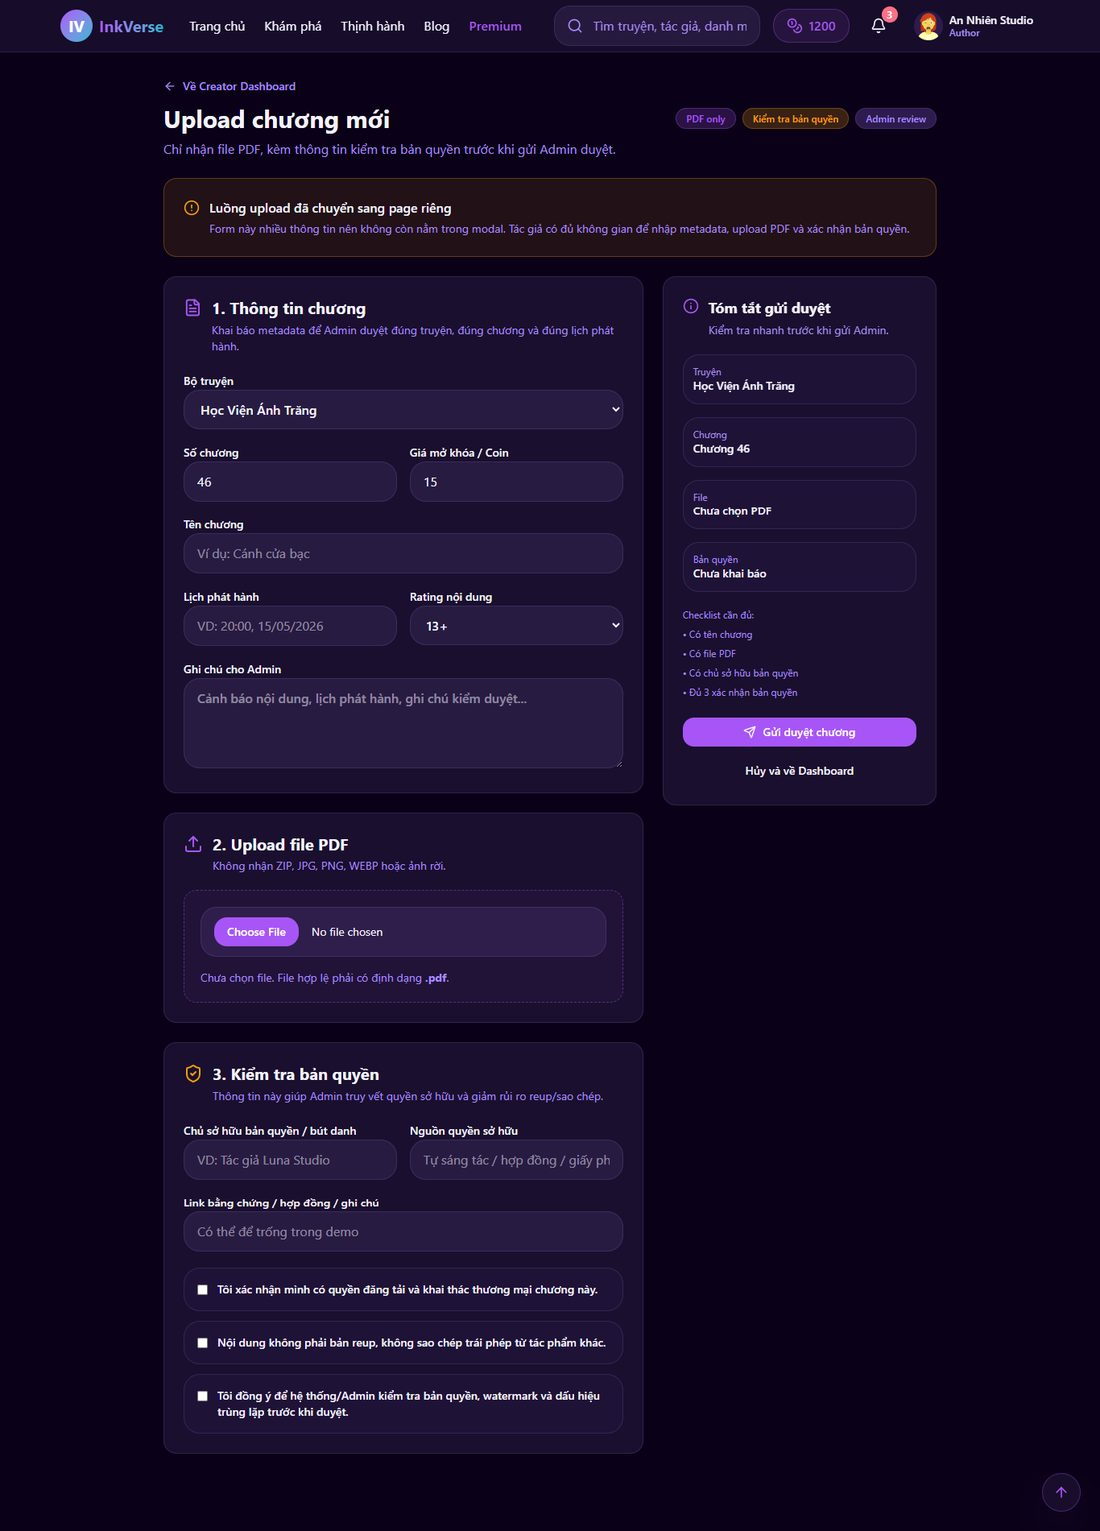
\includegraphics[width=\linewidth,height=0.31\textheight,keepaspectratio]{images/Mockups/author_upload.jpg}
    \scriptsize Upload
\end{minipage}\hfill
\begin{minipage}{0.32\textwidth}
    \centering
    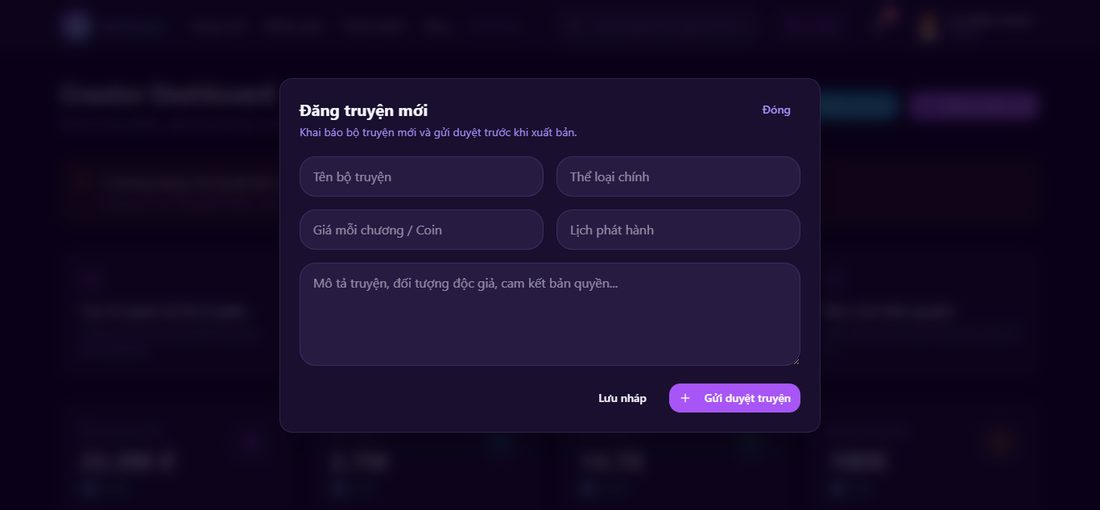
\includegraphics[width=\linewidth,height=0.31\textheight,keepaspectratio]{images/Mockups/author_publish.jpg}
    \scriptsize Publish
\end{minipage}
\caption{Mockup luồng quản lý và xuất bản truyện của tác giả}
\label{fig:mockup-author-publish}
\end{figure}

Dashboard tác giả thể hiện các chỉ số tổng quan như lượt đọc, doanh thu, tác phẩm và hiệu suất nội dung. Màn hình Upload hỗ trợ nhập thông tin truyện hoặc chương, chọn file, mô tả nội dung và các thiết lập liên quan. Modal Publish giúp xác nhận trước khi xuất bản, hạn chế lỗi đăng nhầm hoặc thiếu thông tin.

\begin{figure}[H]
\centering
\begin{minipage}{0.45\textwidth}
    \centering
    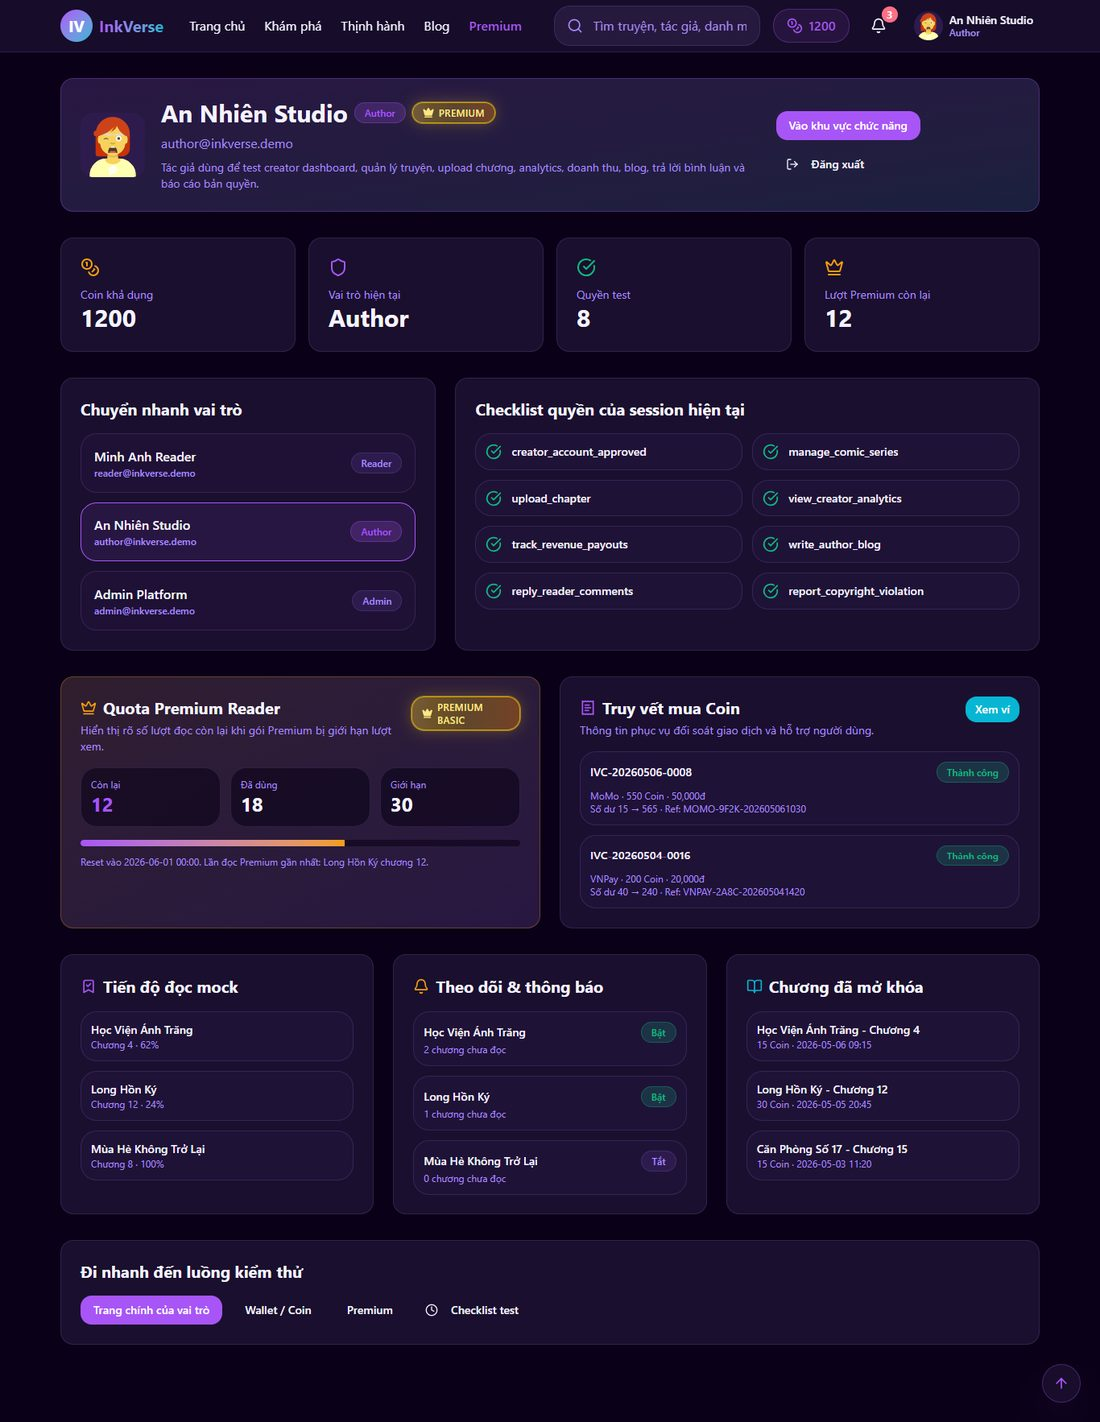
\includegraphics[width=\linewidth,height=0.34\textheight,keepaspectratio]{images/Mockups/author_profile.jpg}
    \scriptsize Author Profile
\end{minipage}\hfill
\begin{minipage}{0.45\textwidth}
    \centering
    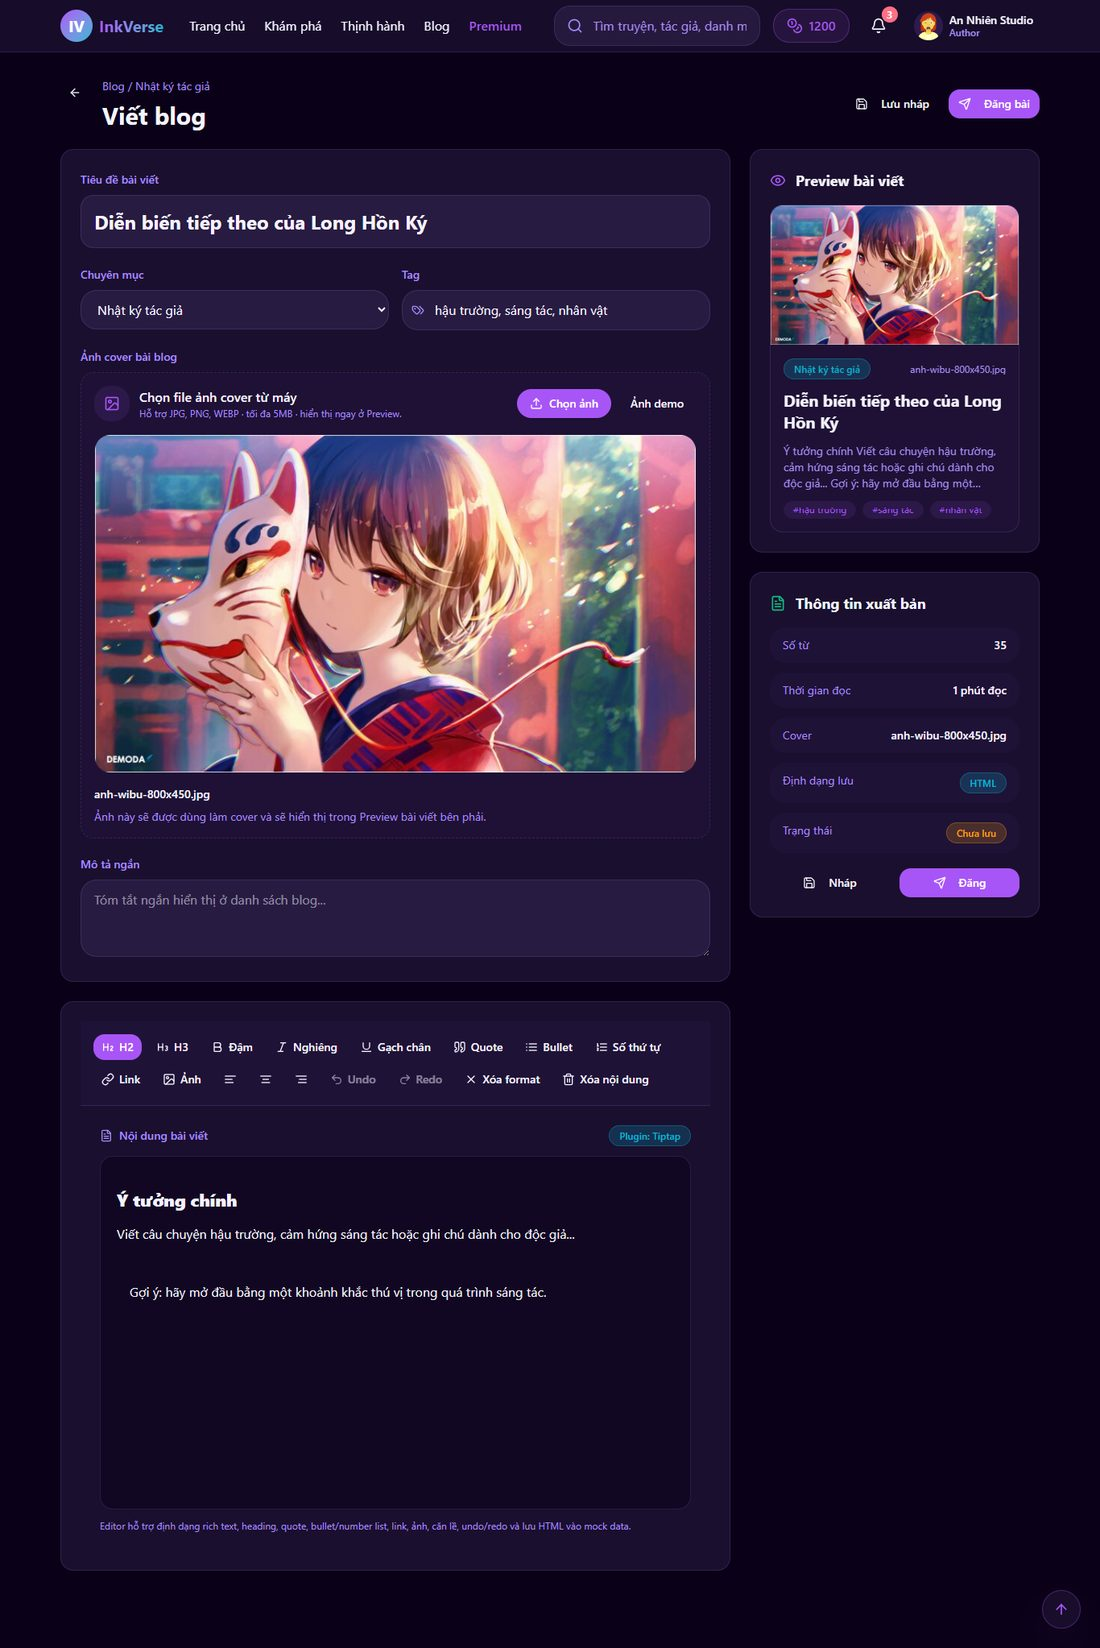
\includegraphics[width=\linewidth,height=0.34\textheight,keepaspectratio]{images/Mockups/author_write_blog.jpg}
    \scriptsize Write Blog
\end{minipage}
\caption{Mockup hồ sơ tác giả và chức năng viết blog}
\label{fig:mockup-author-community}
\end{figure}

Hồ sơ tác giả giúp độc giả nhận diện người sáng tạo, xem tác phẩm và theo dõi hoạt động. Chức năng viết blog mở rộng vai trò của tác giả từ người đăng truyện sang người xây dựng cộng đồng, giúp tăng sự gắn bó giữa tác giả và độc giả.

\subsubsection{Nhóm màn hình Admin}

Nhóm Admin phục vụ vận hành hệ thống. Giao diện admin cần ưu tiên tính rõ ràng, khả năng quan sát số liệu và thao tác quản trị nhanh. Khác với giao diện Reader thiên về cảm xúc đọc, giao diện Admin cần nhiều bảng, chỉ số, trạng thái và bộ lọc để hỗ trợ kiểm duyệt, quản lý người dùng, theo dõi doanh thu và cấu hình nền tảng.

\begin{figure}[H]
\centering
\begin{minipage}{0.45\textwidth}
    \centering
    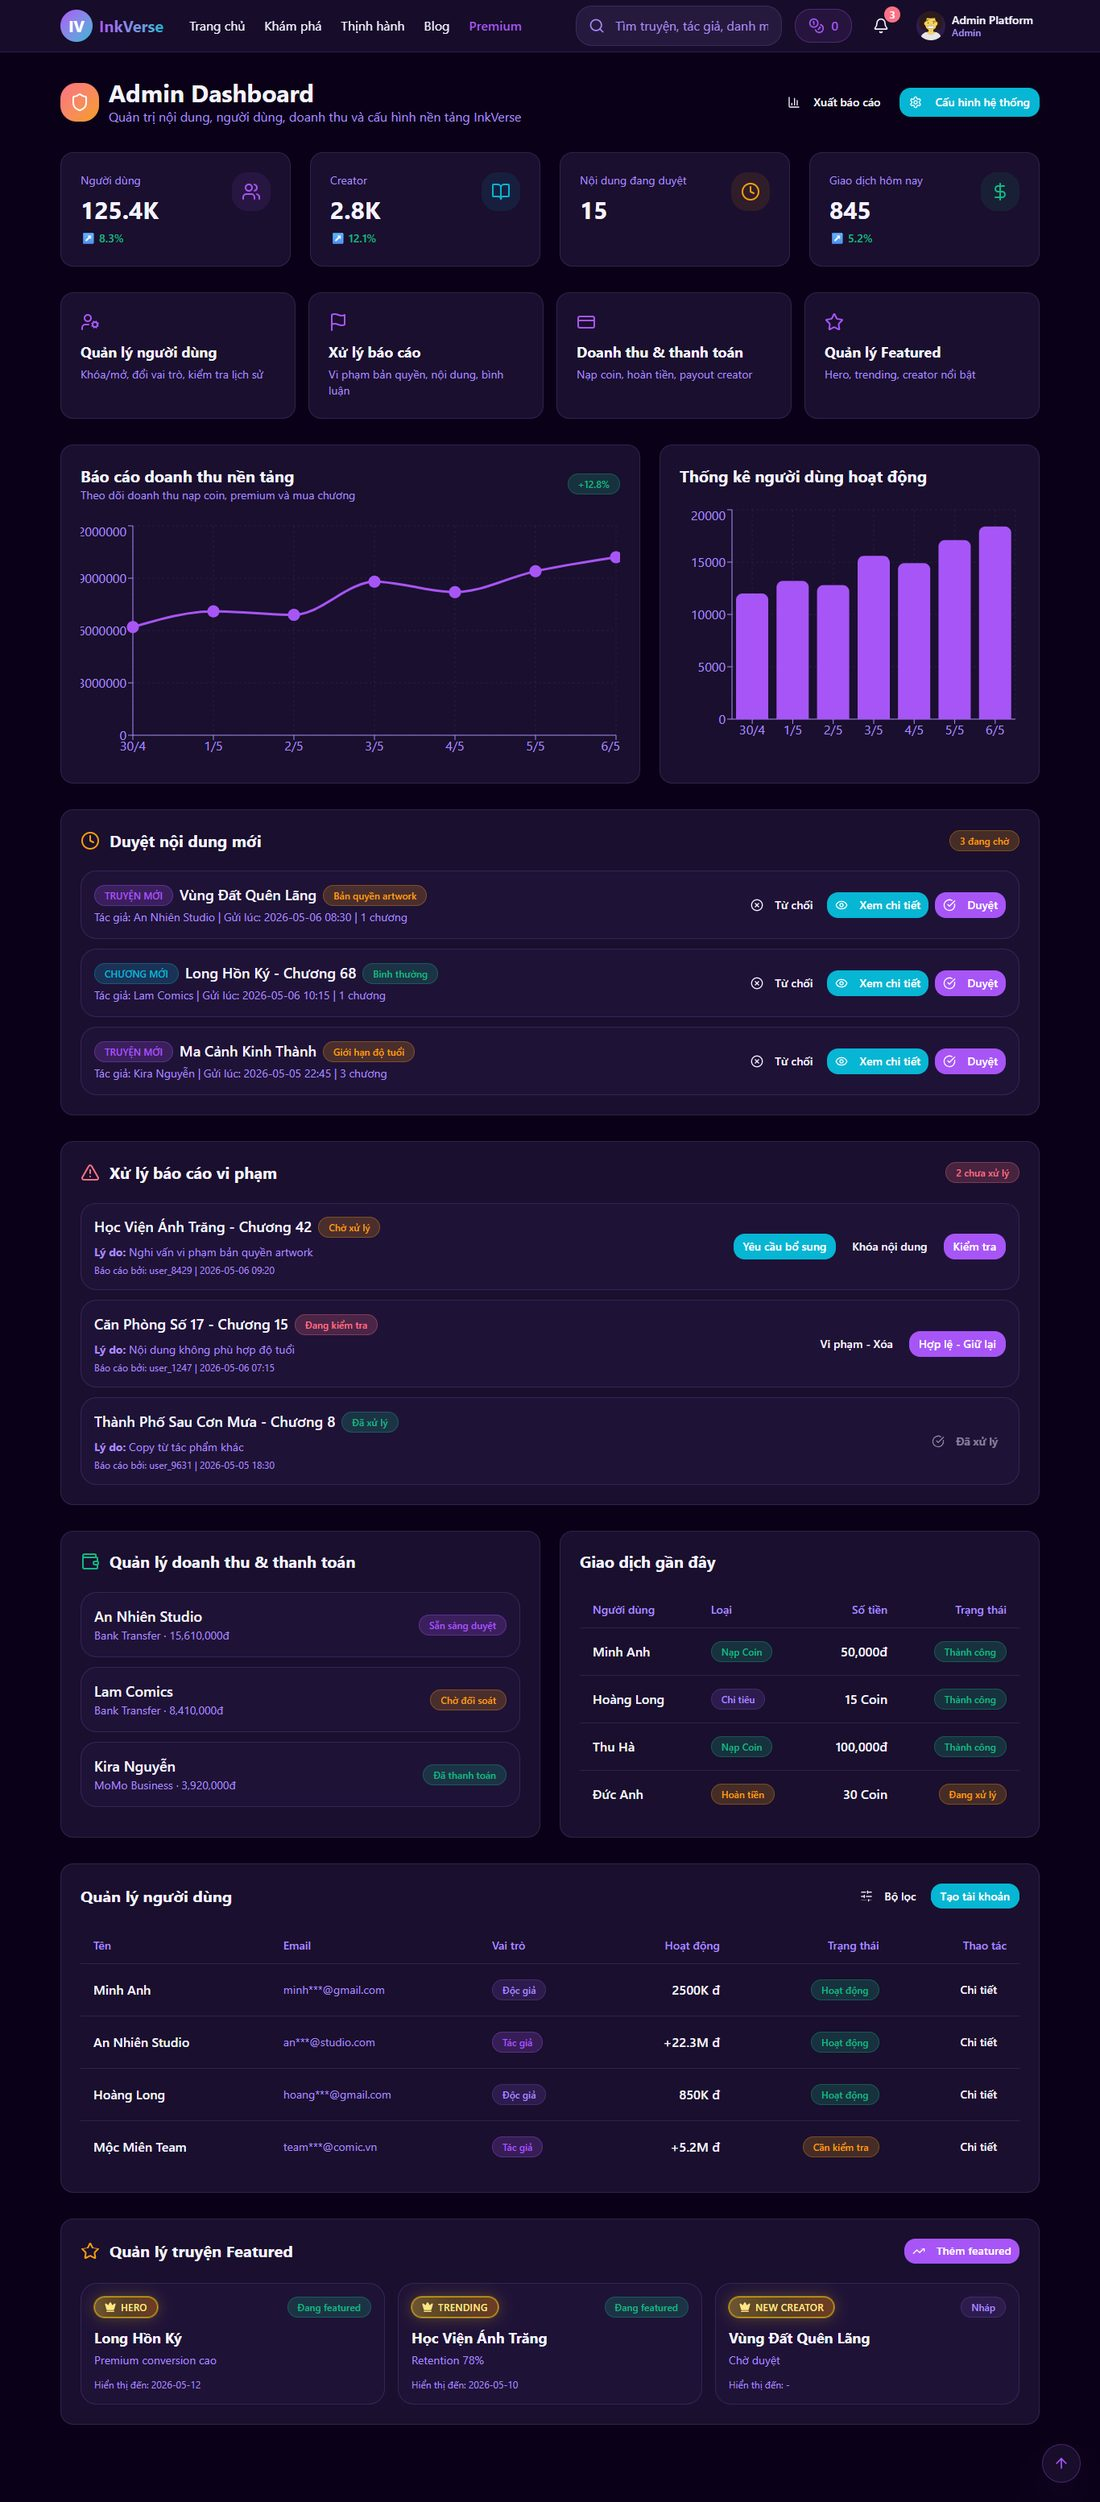
\includegraphics[width=\linewidth,height=0.38\textheight,keepaspectratio]{images/Mockups/admin_dashboard.jpg}
    \scriptsize Admin Dashboard
\end{minipage}\hfill
\begin{minipage}{0.45\textwidth}
    \centering
    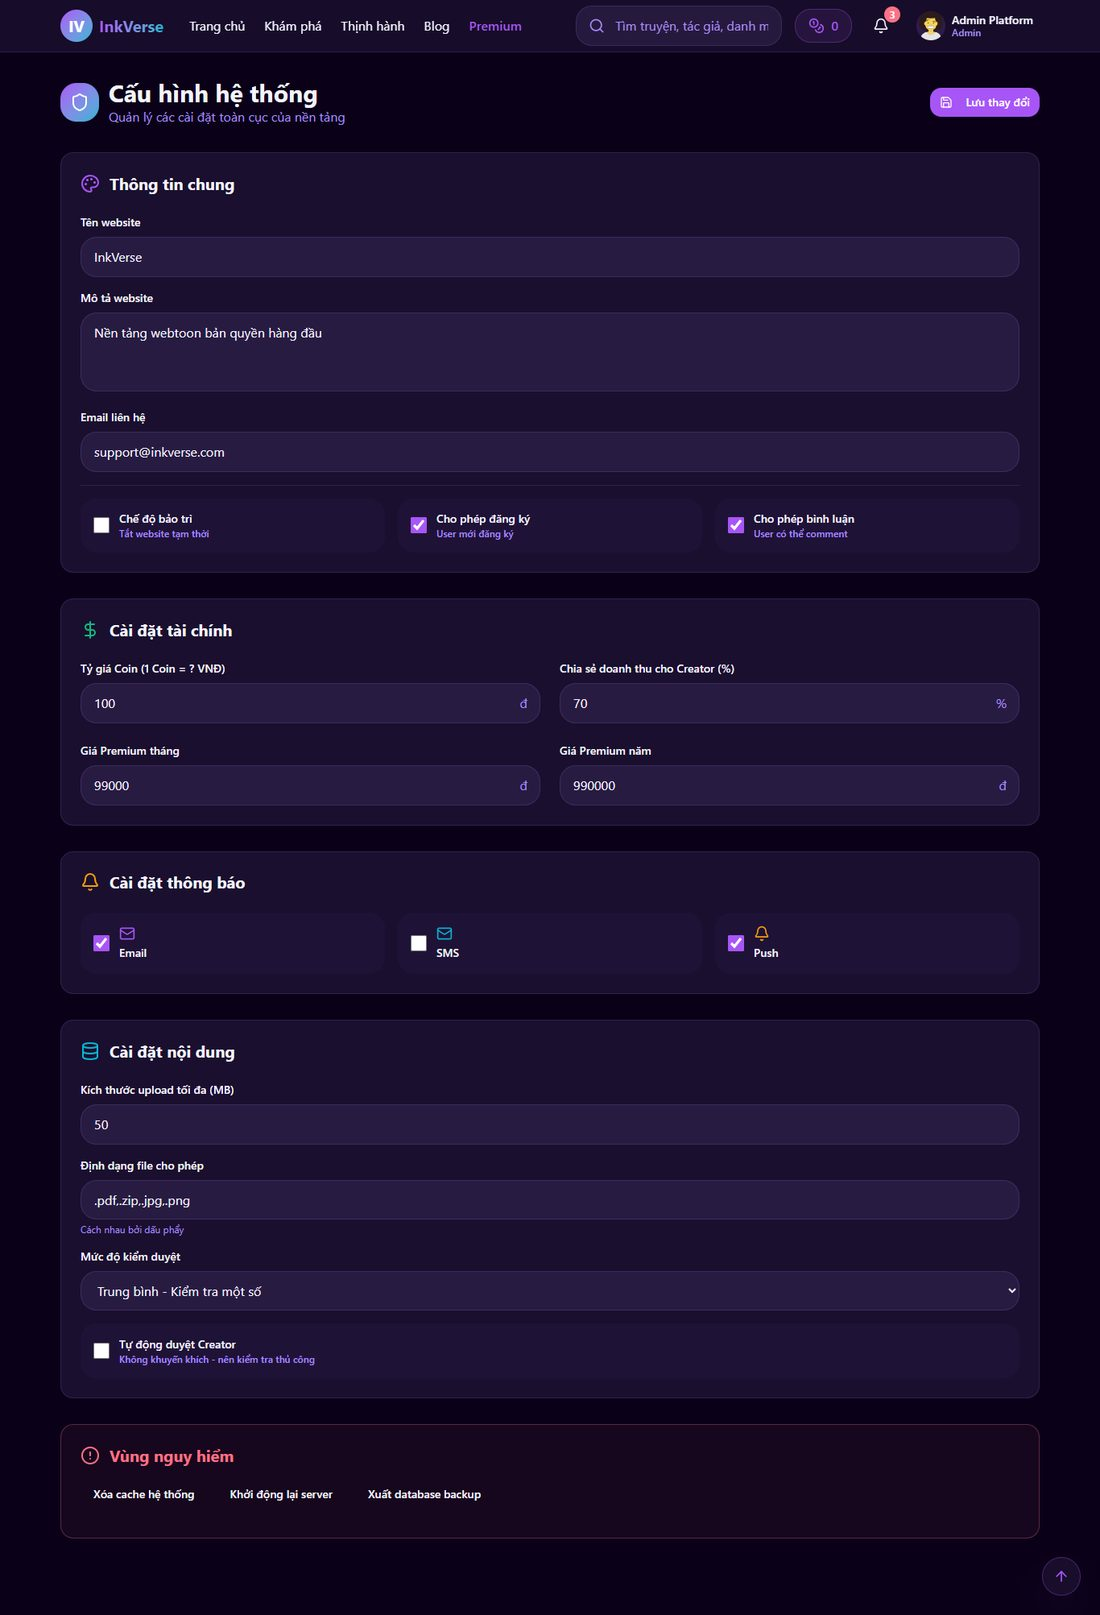
\includegraphics[width=\linewidth,height=0.38\textheight,keepaspectratio]{images/Mockups/admin_settings.jpg}
    \scriptsize Settings
\end{minipage}
\caption{Mockup màn hình quản trị hệ thống}
\label{fig:mockup-admin}
\end{figure}

Dashboard admin tổng hợp các chỉ số như người dùng, doanh thu, tác phẩm, hoạt động gần đây và trạng thái kiểm duyệt. Màn hình Settings cho phép cấu hình thông tin nền tảng, chính sách thanh toán, thông báo và các thông số hệ thống. Việc tách khu vực quản trị khỏi giao diện độc giả giúp bảo đảm hệ thống có thể mở rộng vận hành khi số lượng truyện, giao dịch và người dùng tăng lên.

\subsection{Đánh giá luồng trải nghiệm tổng thể}

Từ các mockup trên, luồng UI/UX có thể được tóm tắt thành bốn hành trình chính:

\begin{enumerate}
    \item \textbf{Hành trình khám phá}: người dùng vào Home, xem các truyện nổi bật, chuyển sang Explore để lọc theo thể loại, sau đó vào Comic Detail để xem mô tả và danh sách chương.
    \item \textbf{Hành trình đọc và trả phí}: người dùng đọc chương, gặp chương trả phí, xem modal Buy Comic, xác nhận Payment, sau đó quay lại màn hình đọc với trạng thái đã sở hữu.
    \item \textbf{Hành trình giữ chân}: người dùng lưu truyện vào Library, quản lý Wallet, xem lịch sử giao dịch và cập nhật Profile. Đây là nhóm chức năng giúp tăng tần suất quay lại nền tảng.
    \item \textbf{Hành trình xuất bản}: tác giả vào Dashboard, upload nội dung, publish chương, viết blog và theo dõi hiệu quả. Hành trình này giúp nền tảng có nguồn cung nội dung ổn định hơn.
\end{enumerate}

Nhìn chung, mockup đã bám khá sát mô hình kinh doanh của nền tảng truyện tranh số: đọc miễn phí có giới hạn, mua chương, ví điện tử, Premium, cộng đồng và dashboard tác giả. Điểm mạnh là hệ thống giao diện nhất quán về màu sắc, card nội dung và phân tách vai trò. Điểm cần tiếp tục hoàn thiện ở giai đoạn hiện thực là bổ sung trạng thái lỗi, trạng thái rỗng, skeleton loading, responsive mobile chi tiết và các thông báo bảo vệ người dùng khi thanh toán thất bại. Nếu các trạng thái này được xử lý tốt, UI/UX sẽ không chỉ đẹp về mặt trình bày mà còn hỗ trợ trực tiếp cho độ tin cậy và khả năng chuyển đổi của sản phẩm.

\section{Kiến trúc hệ thống}
\subsection{System Architecture Diagram}

Hệ thống nền tảng truyện tranh số được xây dựng theo kiến trúc \textbf{Modular Monolith} (Monolith dạng Module). Trong kiến trúc này, hệ thống được chia thành các phân hệ chức năng độc lập về mặt logic nhưng cùng vận hành trong một đơn vị triển khai duy nhất. Đặc biệt, mỗi module bên trong lại được tổ chức theo mô hình \textbf{Kiến trúc phân lớp (Layered Architecture)} để đảm bảo tính tách biệt của các thành phần (Separation of Concerns).

\begin{figure}[htbp]
    \centering
    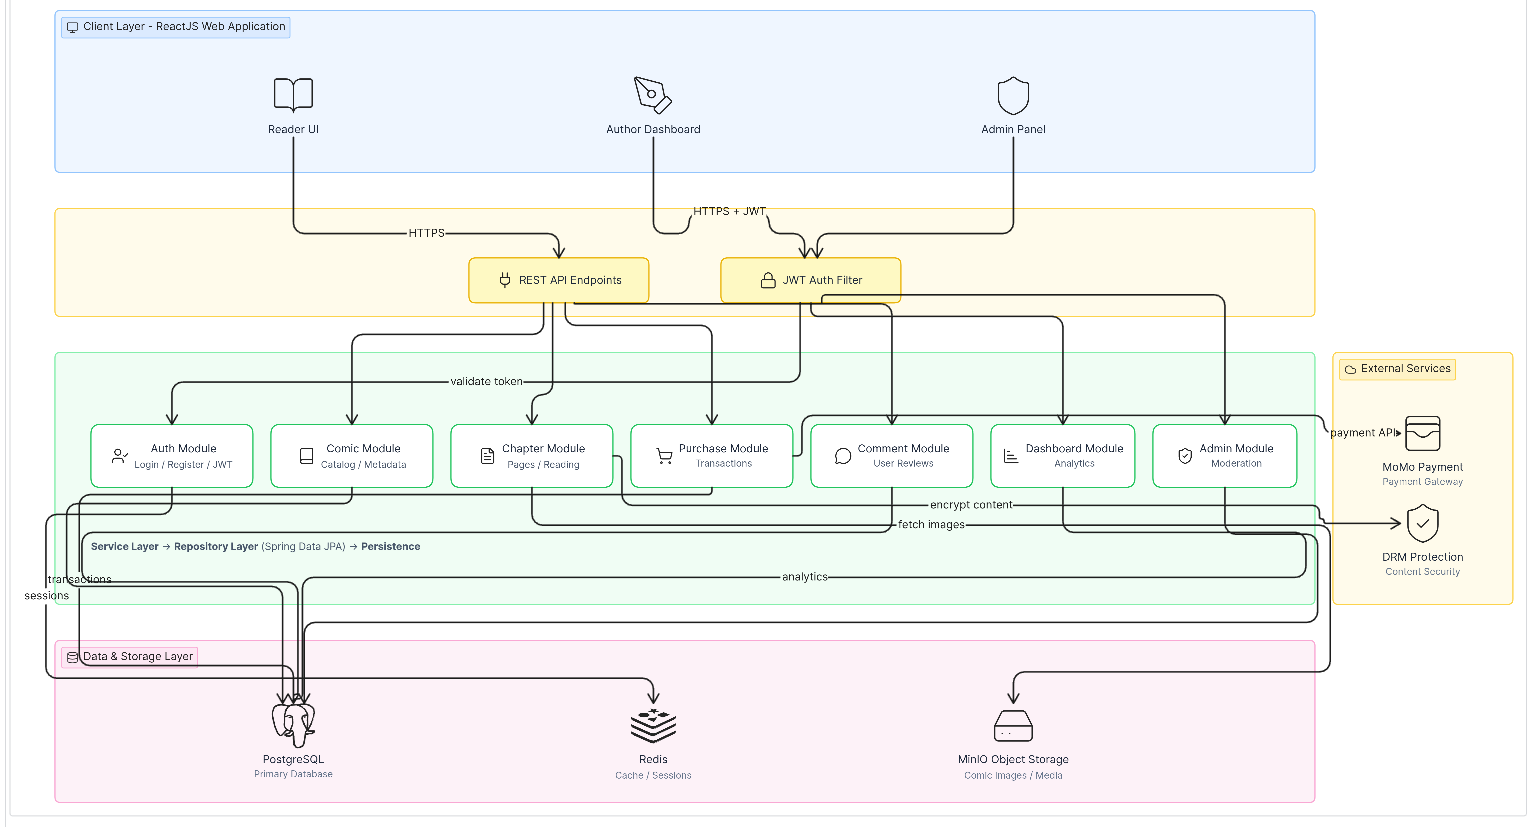
\includegraphics[width=\textwidth]{images/Diagram/architecture.png}
    \caption{Biểu đồ kiến trúc tổng thể của hệ thống}
    \label{fig:system_architecture}
\end{figure}

Dựa vào biểu đồ kiến trúc ở Hình \ref{fig:system_architecture}, hệ thống được cấu thành từ 4 lớp chính và 1 khối dịch vụ bên ngoài:

\subsubsection{Tầng Client (Client Layer - ReactJS Web Application)}
Tầng này đóng vai trò là giao diện tiếp xúc trực tiếp với người dùng, được xây dựng hoàn toàn dưới dạng Ứng dụng Web Single Page Application (SPA) sử dụng \textbf{ReactJS}. Tầng này được chia thành 3 nhóm giao diện chuyên biệt:
\begin{itemize}
    \item \textbf{Reader UI:} Giao diện công cộng dành cho độc giả để tìm kiếm, đọc truyện và thực hiện giao dịch mua. Luồng này giao tiếp qua giao thức HTTPS thông thường tới các API công khai.
    \item \textbf{Author Dashboard:} Trang quản trị dành riêng cho tác giả để tải lên các chương truyện mới, xem thống kê lượt đọc và quản lý doanh thu. Luồng này yêu cầu mức độ bảo mật cao hơn (HTTPS + JWT).
    \item \textbf{Admin Panel:} Màn hình quản lý nội bộ dành cho ban quản trị để kiểm duyệt nội dung, quản lý người dùng và xử lý báo cáo vi phạm (yêu cầu HTTPS + JWT).
\end{itemize}

\subsubsection{Tầng Giao tiếp và Bảo mật (API \& Security Gateway)}
Làm nhiệm vụ tiếp nhận, định tuyến và kiểm tra các yêu cầu (requests) từ phía Client trước khi chuyển xuống tầng xử lý nghiệp vụ:
\begin{itemize}
    \item \textbf{REST API Endpoints:} Đảm nhận việc nhận các API call. Các chức năng đọc công khai sẽ đi trực tiếp qua đây xuống tầng Dịch vụ.
    \item \textbf{JWT Auth Filter:} Đóng vai trò là màng lọc bảo mật khắt khe. Nó kiểm tra tính hợp lệ của token (JWT) cho các API yêu cầu quyền truy cập (như sửa/xóa truyện, giao dịch mua, quyền quản trị). Nếu token hợp lệ (\textit{validate token}), luồng dữ liệu mới được phép đi tiếp.
\end{itemize}

\subsubsection{Tầng Dịch vụ (Service Layer)}
Đây là tầng cốt lõi chứa toàn bộ logic nghiệp vụ (Business Logic) của nền tảng. Nhằm tối ưu hóa khả năng bảo trì và mở rộng, tầng này được tổ chức theo mô hình \textbf{Modular Monolith}, chia thành các module chức năng độc lập. Mỗi module (ví dụ: \texttt{comic}, \texttt{auth}, \texttt{payment}...) lại được xây dựng theo kiến trúc \textbf{Layered} nội bộ bao gồm:
\begin{itemize}
    \item \textbf{Controller Layer:} Tiếp nhận các yêu cầu HTTP/REST API, xử lý đầu vào và điều hướng yêu cầu.
    \item \textbf{Service Layer:} Nơi chứa toàn bộ các quy tắc và logic nghiệp vụ chính của module.
    \item \textbf{Repository Layer:} Sử dụng Spring Data JPA để tương tác với cơ sở dữ liệu PostgreSQL.
    \item \textbf{Domain/DTO Layer:} Chứa các thực thể (Entities) ánh xạ với database, các đối tượng truyền tải dữ liệu (DTO) và Mapper để chuyển đổi dữ liệu an toàn giữa các lớp.
\end{itemize}

Các module chính trong hệ thống bao gồm:
\begin{itemize}
    \item \textbf{Auth Module:} Xử lý các nghiệp vụ đăng nhập (Login), đăng ký (Register) và cấp phát/quản lý JWT.
    \item \textbf{Comic Module:} Quản lý danh mục (Catalog) và siêu dữ liệu (Metadata) của các bộ truyện.
    \item \textbf{Chapter Module:} Quản lý nội dung các trang truyện (Pages) và tối ưu hóa luồng tải trang khi đọc (Reading).
    \item \textbf{Purchase/Payment Module:} Xử lý các giao dịch (Transactions) mua chương truyện và tích hợp cổng thanh toán MoMo.
    \item \textbf{Comment Module:} Quản lý hệ thống đánh giá, phản hồi (User Reviews) của người dùng.
    \item \textbf{Dashboard Module:} Cung cấp và tổng hợp các số liệu phân tích (Analytics) phục vụ cho biểu đồ của tác giả/admin.
    \item \textbf{Admin Module:} Hỗ trợ các công cụ kiểm duyệt nội dung (Moderation).
\end{itemize}

\subsubsection{Tầng Lưu trữ Dữ liệu (Data \& Storage Layer)}
Đảm nhiệm vai trò lưu trữ toàn bộ dữ liệu của hệ thống, bao gồm 3 nền tảng lưu trữ chuyên biệt để tối ưu cho từng loại dữ liệu:
\begin{itemize}
    \item \textbf{PostgreSQL (Primary Database):} Cơ sở dữ liệu quan hệ chính, lưu trữ an toàn các dữ liệu có cấu trúc quan trọng (thông tin người dùng, chi tiết giao dịch, thông tin truyện).
    \item \textbf{Redis (Cache / Sessions):} Sử dụng làm bộ nhớ đệm tốc độ cao để lưu trữ các phiên làm việc (sessions) của người dùng, đồng thời cache các dữ liệu được truy vấn thường xuyên (như danh sách truyện thịnh hành và siêu dữ liệu truyện) nhằm giảm tải tối đa cho Database chính.
    \item \textbf{MinIO Object Storage:} Hệ thống lưu trữ hướng đối tượng, chuyên dùng để lưu trữ và phân phối khối lượng lớn các tệp tin hình ảnh truyện (Comic Images/Media), giúp tối ưu tốc độ tải ảnh.
\end{itemize}

\subsubsection{Các dịch vụ bên ngoài (External Services)}
Hệ thống linh hoạt tích hợp các dịch vụ của bên thứ ba để hoàn thiện hệ sinh thái:
\begin{itemize}
    \item \textbf{MoMo Payment Gateway:} Tích hợp thông qua \textit{payment API} để hỗ trợ độc giả thanh toán điện tử tiện lợi khi nạp xu hoặc mua truyện trả phí.
    \item \textbf{DRM Protection (Content Security):} Dịch vụ mã hóa và bảo vệ bản quyền nội dung (Encrypt content). Các hình ảnh truyện trước khi trả về cho client có thể đi qua lớp DRM để ngăn chặn các hành vi tải lậu hoặc chụp ảnh màn hình trái phép, bảo vệ quyền lợi chính đáng của tác giả.
\end{itemize}

\section{Công nghệ Stack triển khai}

Dựa trên yêu cầu và thiết kế kiến trúc thực tế, hệ thống sử dụng các công nghệ sau cho từng phân lớp:

\subsubsection{Tầng Presentation (Frontend)}
\begin{itemize}
    \item \textbf{React (Vite):} Được sử dụng làm nền tảng xây dựng giao diện, tập trung vào hiệu năng rendering và mang lại khả năng tương tác mượt mà cho người dùng.
    \item \textbf{Đặc điểm kỹ thuật:} Tầng này giao tiếp với hệ thống qua RESTful API chuẩn hóa và bảo mật xác thực thông qua JWT Interceptors. Sử dụng TypeScript để đảm bảo an toàn về kiểu dữ liệu và Tailwind CSS kết hợp với Radix UI để xây dựng giao diện hiện đại.
\end{itemize}

\subsubsection{Tầng Business (Backend \& Logic nghiệp vụ)}
\begin{itemize}
    \item \textbf{Java 21 \& Spring Boot 3.4:} Sử dụng các tính năng mới nhất của Java và Spring Boot để tối ưu hiệu năng và khả năng bảo trì.
    \item \textbf{Kiến trúc Modular Monolith:} Backend được thiết kế theo kiến trúc Modular Monolith, chia thành các phân hệ độc lập. Mỗi phân hệ lại tuân thủ mô hình \textbf{Layered Architecture} (Controller - Service - Repository) để tách biệt logic xử lý.
    \item \textbf{Cơ chế phân quyền (RBAC - Role-Based Access Control):} Hệ thống phân quyền chặt chẽ với các vai trò (Role) chính: \textit{Reader, Author, Admin}.
\end{itemize}

\subsubsection{Tầng Data (Cơ sở dữ liệu)}
\begin{itemize}
    \item \textbf{PostgreSQL:} Được lựa chọn làm cơ sở dữ liệu quan hệ chính để đảm bảo sự tin cậy tuyệt đối cho dữ liệu.
    \item \textbf{Ưu điểm áp dụng:} Hệ quản trị này tuân thủ tính ACID, đảm bảo các giao dịch mua chương truyện không bao giờ gặp lỗi trạng thái. PostgreSQL tối ưu hóa tốc độ tìm kiếm truyện (theo tên, tác giả, thể loại) thông qua Indexing  và sẵn sàng cho khả năng mở rộng (Scalability) bằng cơ chế Replication (Master-Slave).
\end{itemize}

\subsubsection{Lưu trữ tài nguyên (Object Storage)}
\begin{itemize}
    \item \textbf{MinIO:} Hệ thống sử dụng MinIO làm Object Storage chuyên dụng thay vì lưu trữ file trực tiếp trong Server hoặc Database.
    \item \textbf{Ưu điểm áp dụng:} MinIO đáp ứng hiệu suất cao khi phải phục vụ hàng triệu tệp tin hình ảnh trang truyện. Việc hỗ trợ chuẩn S3 API giúp hệ thống dễ dàng chuyển đổi sang AWS S3 hoặc Google Cloud Storage trong tương lai. Quan trọng nhất, tài nguyên được bảo mật nội dung trả phí thông qua cơ chế Signed URLs.
\end{itemize}

\subsubsection{Tối ưu hiệu năng (Caching)}
\begin{itemize}
    \item \textbf{Redis:} Đóng vai trò là hệ thống lưu trữ in-memory để tối ưu hiệu năng.
    \item \textbf{Chức năng chính:} Redis hoạt động như một hệ thống lưu trữ in-memory phục vụ hai vai trò cốt lõi là quản lý phiên làm việc (sessions) của người dùng và lưu trữ dữ liệu đệm (cache). Cụ thể, hệ thống sử dụng Redis để duy trì trạng thái phiên đăng nhập, lưu trữ danh sách truyện thịnh hành ("Hot Comics"), và cache siêu dữ liệu (metadata) của những bộ truyện có lượt xem cao nhằm phục vụ nhanh các truy vấn thường xuyên và giảm tải hệ thống đáng kể.
\end{itemize}

\subsection{Thiết kế Cơ sở dữ liệu (ER Diagram)}

Biểu đồ Thực thể - Mối kết hợp (ERD - Entity Relationship Diagram) ở Hình \ref{fig:erd} mô tả cấu trúc dữ liệu tổng thể của nền tảng. Các thực thể và mối quan hệ được thiết kế tối ưu để phục vụ cho các luồng nghiệp vụ cốt lõi: đọc truyện, quản lý người dùng, tương tác cộng đồng và đặc biệt là hệ thống thanh toán vi mô (micro-transaction). Dựa theo ERD, có thể phân nhóm các thực thể thành 4 nhóm chính.

\begin{figure}[htbp]
    \centering
    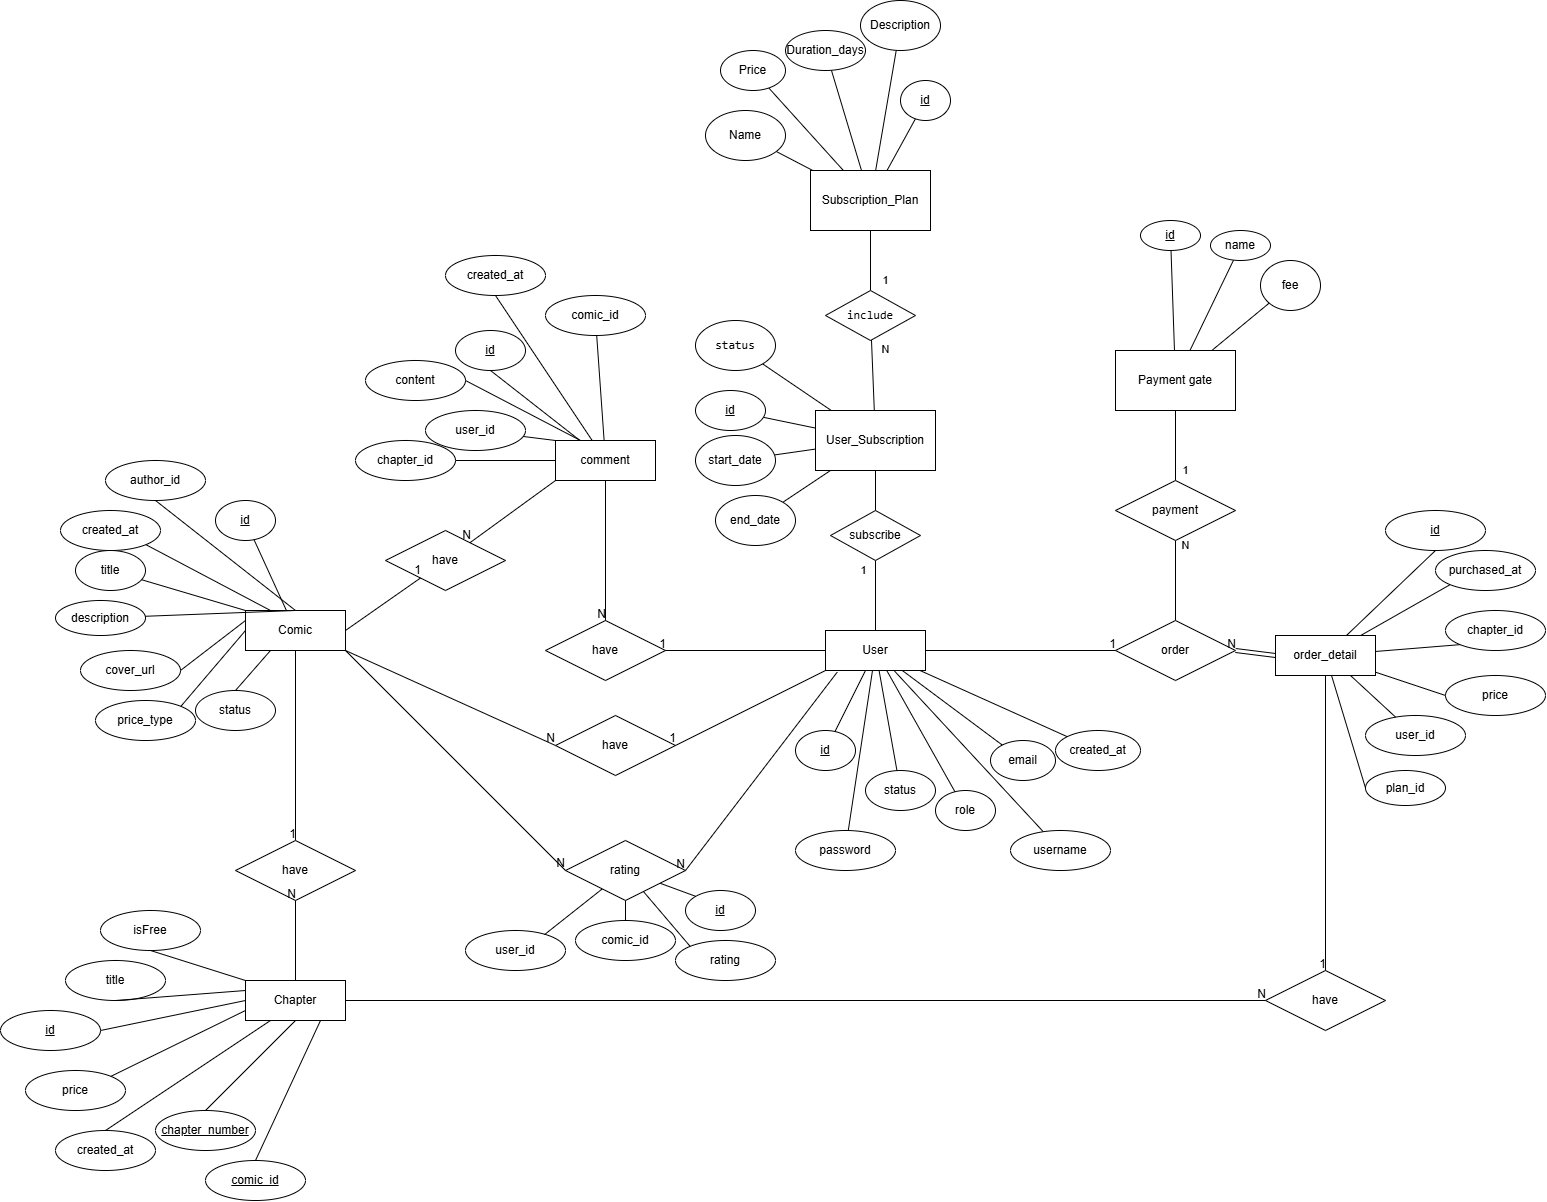
\includegraphics[width=\textwidth]{images/Diagram/TMĐT-erd.png}
    \caption{Biểu đồ Thực thể - Mối kết hợp (ERD) của hệ thống}
    \label{fig:erd}
\end{figure}

\subsubsection{Nhóm Quản lý Người dùng (User)}
\begin{itemize}
    \item \textbf{\texttt{User}:} Bảng trung tâm lưu trữ thông tin tài khoản của tất cả người dùng trên hệ thống (bao gồm các thuộc tính: \textit{id, username, password, email, role, status, created\_at}). Trường \texttt{role} đóng vai trò quan trọng trong việc phân quyền RBAC (Role-Based Access Control) giữa Độc giả, Tác giả và Quản trị viên (Admin).
\end{itemize}

\subsubsection{Nhóm Quản lý Nội dung (Comic \& Chapter)}
\begin{itemize}
    \item \textbf{\texttt{Comic}:} Lưu trữ thông tin tổng quan của một bộ truyện (\textit{id, title, description, cover\_url, price\_type, status}). Thực thể này có liên kết tới tài khoản sáng tác thông qua trường \texttt{author\_id}.
    \item \textbf{\texttt{Chapter}:} Chi tiết các chương thuộc một bộ truyện (\textit{chapter\_number, title, isFree, price}). Một \texttt{Comic} có mối quan hệ 1-N (Một - Nhiều) với \texttt{Chapter}. Thuộc tính \texttt{isFree} (True/False) kết hợp với \texttt{price} giúp hệ thống xác định nhanh chóng các chương đọc miễn phí và các chương bị khóa (paywall) cần trả phí.
\end{itemize}

\subsubsection{Nhóm Giao dịch \& Doanh thu (Order \& Subscription)}
Nhóm này được thiết kế linh hoạt để hỗ trợ cùng lúc hai mô hình kinh doanh cốt lõi (Mua lẻ và Đăng ký gói):
\begin{itemize}
    \item \textbf{\texttt{Subscription\_Plan} \& \textbf{\texttt{User\_Subscription}}:} Quản lý các gói hội viên (Premium). \texttt{Subscription\_Plan} lưu thông tin gói (\textit{Name, Price, Duration\_days}), trong khi \texttt{User\_Subscription} là bảng trung gian ghi nhận thời hạn sử dụng của người dùng (\textit{start\_date, end\_date, status}).
    \item \textbf{\texttt{Payment\_gate}:} Danh mục các cổng thanh toán tích hợp (ví dụ: MoMo, ZaloPay, v.v.) và mức phí giao dịch (\textit{fee}).
    \item \textbf{\texttt{Order} \& \textbf{\texttt{Order\_detail}}:} Quản lý hóa đơn. Một giao dịch (\texttt{Order}) được gắn với một \texttt{User} và một \texttt{Payment\_gate}. Chi tiết giao dịch (\texttt{Order\_detail}) sẽ trỏ khóa ngoại tới \texttt{chapter\_id} (nếu người dùng mua lẻ chương) hoặc \texttt{plan\_id} (nếu người dùng mua gói Premium), kèm theo giá tiền (\textit{price}) tại thời điểm mua để đảm bảo tính nhất quán của dữ liệu tài chính.
\end{itemize}

\subsubsection{Nhóm Tương tác Cộng đồng (Comment \& Rating)}
\begin{itemize}
    \item \textbf{\texttt{Rating}:} Bảng trung gian thể hiện mối quan hệ nhiều-nhiều (N - N) giữa \texttt{User} và \texttt{Comic}. Mỗi bản ghi lưu trữ điểm số (\textit{rating}) mà một người dùng đánh giá cho một bộ truyện cụ thể.
    \item \textbf{\texttt{Comment}:} Lưu trữ bình luận của người dùng (\textit{content, created\_at}). Thiết kế hỗ trợ khóa ngoại trỏ tới cả \texttt{comic\_id} và \texttt{chapter\_id}, cho phép độc giả linh hoạt bình luận cho tổng thể toàn bộ truyện hoặc thảo luận chi tiết theo từng chương riêng biệt.
\end{itemize}

\subsection{Khả năng mở rộng (Scalability)}

Để đảm bảo hệ thống vận hành ổn định và giữ vững hiệu năng khi số lượng độc giả và tác giả tăng trưởng đột biến, kiến trúc nền tảng được thiết kế tối ưu cho khả năng mở rộng linh hoạt ở cả tầng xử lý nghiệp vụ, tầng lưu trữ tài nguyên tĩnh và tầng cơ sở dữ liệu. Khả năng mở rộng của hệ thống được xây dựng dựa trên các trụ cột công nghệ cốt lõi sau:

\subsubsection{Mở rộng tầng lưu trữ tài nguyên tĩnh (Media Storage Scalability)}
Đối với một nền tảng truyện tranh số, hình ảnh của từng trang truyện là loại tài nguyên chiếm dung lượng lớn nhất và yêu cầu băng thông phân phối cực cao. Việc sử dụng hệ thống lưu trữ hướng đối tượng giải quyết bài toán mở rộng này một cách triệt để:
\begin{itemize}
    \item \textbf{Tách rời tài nguyên:} Hệ thống sử dụng \texttt{MinIO Object Storage} làm kho lưu trữ chuyên dụng thay vì lưu trực tiếp trong cơ sở dữ liệu quan hệ hoặc ổ đĩa cục bộ của server backend. Thiết kế này cho phép hệ thống phục vụ hàng triệu tệp tin hình ảnh trang truyện mà không làm ảnh hưởng đến hiệu suất xử lý logic nghiệp vụ.
    \item \textbf{Sẵn sàng dịch chuyển lên Cloud:} Nhờ việc hỗ trợ hoàn toàn chuẩn S3 API, hệ thống sở hữu khả năng mở rộng quy mô không giới hạn. Khi lượng truy cập vượt quá khả năng chịu tải của hạ tầng tại chỗ (on-premise), nền tảng có thể chuyển dịch dễ dàng sang các dịch vụ đám mây lớn như AWS S3 hoặc Google Cloud Storage mà không cần phải thay đổi cấu trúc mã nguồn cốt lõi.
\end{itemize}

\subsubsection{Mở rộng và giảm tải tầng dữ liệu (Database Scalability \& Caching)}
Cơ sở dữ liệu thường là điểm nghẽn hệ thống (bottleneck) lớn nhất khi ứng dụng mở rộng. Hệ thống khắc phục bằng cách phân tách luồng xử lý và áp dụng bộ nhớ đệm tốc độ cao:
\begin{itemize}
    \item \textbf{PostgreSQL Replication:} Hệ quản trị cơ sở dữ liệu PostgreSQL được cấu hình sẵn sàng cho cơ chế sao lưu dữ liệu theo mô hình Master-Slave. Mọi tác vụ ghi dữ liệu đòi hỏi tính nhất quán cao như giao dịch tài chính (mua chương, nạp xu) sẽ được xử lý tại nút Master để đảm bảo tính nghiêm ngặt của ACID. Trong khi đó, các tác vụ đọc dữ liệu nặng (truy vấn danh mục truyện, thông tin chương) sẽ được phân tải (load balancing) ra các nút Slave, giúp hệ thống mở rộng khả năng đáp ứng đồng thời cho hàng vạn độc giả cùng lúc.
    \item \textbf{Redis In-Memory Caching:} Hệ thống sử dụng Redis để lưu trữ trạng thái phiên làm việc (sessions) của người dùng và phục vụ trực tiếp các truy vấn dữ liệu phổ biến. Việc cache danh sách truyện thịnh hành ("Hot Comics") và siêu dữ liệu (metadata) của các bộ truyện có lượt xem cao giúp giảm tải tối đa số lượng request phải truy vấn trực tiếp xuống Database chính, từ đó giải phóng tài nguyên để PostgreSQL xử lý các luồng giao dịch cốt lõi một cách mượt mà.
\end{itemize}

\subsubsection{Mở rộng cấu trúc mã nguồn Backend (Architectural Scalability)}
Hệ thống lựa chọn hướng tiếp cận backend theo kiến trúc \textbf{Modular Monolith} nhằm tối ưu hóa khả năng phát triển và mở rộng mã nguồn theo thời gian:
\begin{itemize}
    \item \textbf{Tính cô lập cao:} Mã nguồn được phân chia thành các module chức năng có ranh giới rõ ràng (Auth \& User, Comic \& Chapter, Purchase, Comment). Điều này cho phép đội ngũ kỹ thuật nhỏ dễ dàng phát triển song song các tính năng mới mà không gây ảnh hưởng chéo hoặc làm xung đột mã nguồn hệ thống.
    \item \textbf{Định hướng phát triển thành Microservices:} Ở giai đoạn đầu của dự án, kiến trúc Modular Monolith giúp tối ưu hóa chi phí vận hành và hạ tầng mạng cơ bản. Tuy nhiên, khi hệ thống tăng trưởng đến một quy mô cực lớn và một số module cụ thể (như Module Chapter phục vụ luồng đọc hoặc Module Purchase phục vụ thanh toán vi mô) bị quá tải, thiết kế dạng modular cho phép đội ngũ kỹ thuật dễ dàng bóc tách riêng module đó ra thành một dịch vụ Microservice độc lập. Dịch vụ này sau đó có thể được container hóa (ví dụ: sử dụng Docker/Kubernetes) để mở rộng theo chiều ngang (Horizontal Scaling) một cách nhanh chóng mà không cần phải đập đi xây lại toàn bộ hệ thống.
\end{itemize}
